\documentclass[12pt,]{article}
%\usepackage{lmodern}  Melissa removed to deal with font rendering issue
\usepackage{amssymb,amsmath}
\usepackage{ifxetex,ifluatex}
\usepackage{fixltx2e} % provides \textsubscript

%Melissa removed the following section to deal with font rendering issue
%\ifnum 0\ifxetex 1\fi\ifluatex 1\fi=0 % if pdftex
%  \usepackage[T1]{fontenc}
%  \usepackage[utf8]{inputenc}
%%\else % if luatex or xelatex
%  \ifxetex
%    \usepackage{mathspec}
%  \else
%    \usepackage{fontspec}
%  \fi
%  \defaultfontfeatures{Ligatures=TeX,Scale=MatchLowercase}
%  \newcommand{\euro}{€}
%%%%%%\fi

% use upquote if available, for straight quotes in verbatim environments
\IfFileExists{upquote.sty}{\usepackage{upquote}}{}
% use microtype if available
\IfFileExists{microtype.sty}{%
\usepackage{microtype}
\UseMicrotypeSet[protrusion]{basicmath} % disable protrusion for tt fonts
}{}
\usepackage[margin=1in]{geometry}
\usepackage{hyperref}
\PassOptionsToPackage{usenames,dvipsnames}{color} % color is loaded by hyperref
\hypersetup{unicode=true,
            pdftitle={The Combined Status of Gopher (Sebastes carnatus) and Black-and-Yellow Rockfishes (Sebastes chrysomelas) in U.S. Waters Off California in 2019},
            pdfborder={0 0 0},
            breaklinks=true}
\urlstyle{same}  % don't use monospace font for urls
\usepackage{graphicx,grffile}
\makeatletter
\def\maxwidth{\ifdim\Gin@nat@width>\linewidth\linewidth\else\Gin@nat@width\fi}
\def\maxheight{\ifdim\Gin@nat@height>\textheight\textheight\else\Gin@nat@height\fi}
\makeatother
% Scale images if necessary, so that they will not overflow the page
% margins by default, and it is still possible to overwrite the defaults
% using explicit options in \includegraphics[width, height, ...]{}
\setkeys{Gin}{width=\maxwidth,height=\maxheight,keepaspectratio}
\setlength{\parindent}{0pt}
\setlength{\parskip}{6pt plus 2pt minus 1pt}
\setlength{\emergencystretch}{3em}  % prevent overfull lines
\providecommand{\tightlist}{%
  \setlength{\itemsep}{0pt}\setlength{\parskip}{0pt}}
\setcounter{secnumdepth}{5}

%%% Use protect on footnotes to avoid problems with footnotes in titles
\let\rmarkdownfootnote\footnote%
\def\footnote{\protect\rmarkdownfootnote}

%%% Change title format to be more compact
\usepackage{titling}

% Create subtitle command for use in maketitle
\newcommand{\subtitle}[1]{
  \posttitle{
    \begin{center}\large#1\end{center}
    }
}

\setlength{\droptitle}{-2em}
  \title{The Combined Status of Gopher (\emph{Sebastes carnatus}) and
Black-and-Yellow Rockfishes (\emph{Sebastes chrysomelas}) in U.S. Waters
Off California in 2019}
  \pretitle{\vspace{\droptitle}\centering\huge}
  \posttitle{\par}
  \author{}
  \preauthor{}\postauthor{}
  \date{}
  \predate{}\postdate{}


% This file contains all of the LaTeX packages you may need to compile the document
% Documentation for each package can be found onlines
\usepackage{tabularx}                                             % table environment providing flexibility
\usepackage{caption}                                              % for creating captions  
\usepackage{longtable}                                            % allows tables to span multiple pages
\usepackage{rotating}                                             % allows for sideways tables
\usepackage{float}                                                % floating environments; may not need in rmarkdown
\usepackage{placeins}                                             % keeps floats from moving
\usepackage{indentfirst}                                          % indents first paragraph of a section
\usepackage{mdwtab}                                               % continued float multi-page figure
\usepackage{enumerate}                                            % create lists
\usepackage{hyperref}                                             % highlight cross references
\hypersetup{colorlinks=true, urlcolor=blue, linktoc=page, linkcolor=blue, citecolor=blue} %define referencing colors
%\usepackage{makebox}                                             % make boxes around text
\usepackage[usenames,dvipsnames]{xcolor}                          % color name options
%\usepackage[space]{grffile}                                      % spaces in file name path
\usepackage{soul}                                                 % highlight text
\usepackage{enumitem}                                             % numbered lists
\usepackage{lineno}                                               % Line numbers; comment out for final
\usepackage{upquote}                                              % produce grave accent in latex
\usepackage{verbatim}                                             % produces verbatim results
\usepackage{fancyvrb}                                             % verbatim in a box
%\usepackage{draftwatermark}                                      % places Draft watermark in background; comment out for final
\usepackage{textcomp}                                             % fixes error with packages interfering
\usepackage{lscape}                                               % rotate pages - to allow for landscape longtables
%\pdfinterwordspaceon                                             % fix loss of inter word spacing
\usepackage{cmap}                                                 % fix mapping characters to unicode
\RequirePackage[linewidth = 1]{pdfcomment}                        % pdf comments
\RequirePackage[l2tabu, orthodox]{nag}                            % checks packages related to the accessibility?
\usepackage[inline]{showlabels}                                   % show table and figure labels; comment out for final
%\RequirePackage[tagged]{accessibilityMeta}


\linenumbers                                                      % specify use of line numbers


\definecolor{light-gray}{gray}{.85}                               % define light-gray as a color
%\usepackage[tagged]{accessibility-meta}

 
%\showlabels[\color{mred}]{label}

% Redefines (sub)paragraphs to behave more like sections
\ifx\paragraph\undefined\else
\let\oldparagraph\paragraph
\renewcommand{\paragraph}[1]{\oldparagraph{#1}\mbox{}}
\fi
\ifx\subparagraph\undefined\else
\let\oldsubparagraph\subparagraph
\renewcommand{\subparagraph}[1]{\oldsubparagraph{#1}\mbox{}}
\fi

\begin{document}
\maketitle


\begin{center}
\thispagestyle{empty}


\vspace{.5cm}

%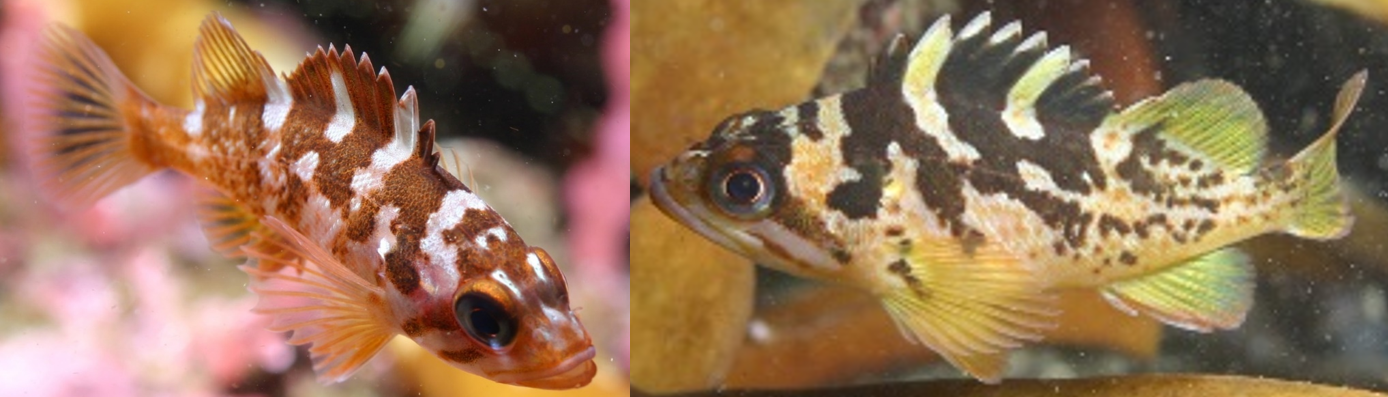
\includegraphics{cover_photo}~\\[1cm]
\pdftooltip{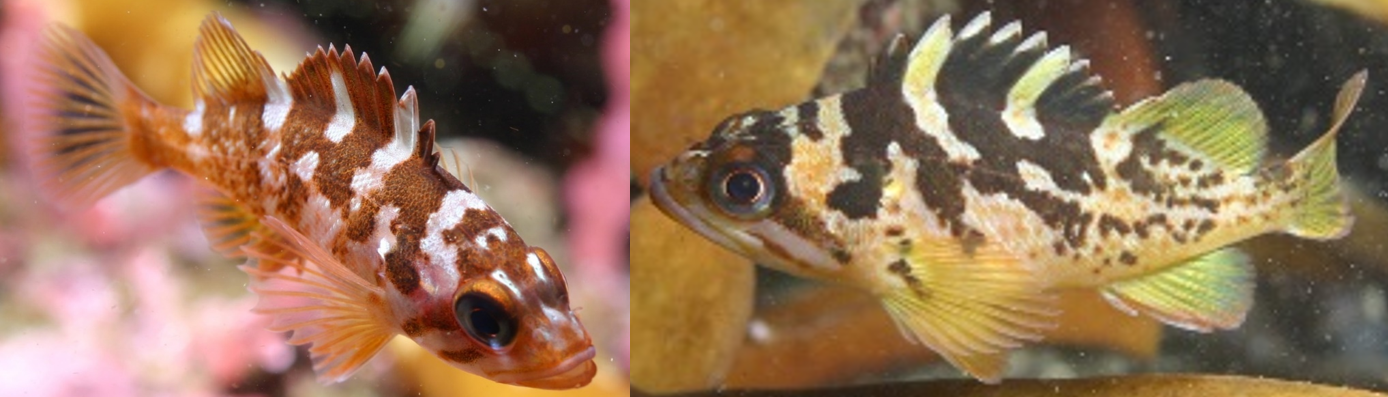
\includegraphics{cover_photo}}{This is a fish.}
Gopher rockfish (left) and black-and-yellow rockfish (right).      
\small
Photos by Steve Lonhart.

\vspace{.3cm}


Melissa H. Monk\textsuperscript{1}\\
Xi He\textsuperscript{1}\\

\vspace{.5cm}

\small
\textsuperscript{1}Southwest Fisheries Science Center, U.S. Department of Commerce, National Oceanic and Atmospheric Administration, National Marine Fisheries Service, 110 McAllister Way, Santa Cruz, California 95060\\

\vspace{1.5cm}


%\vfill
DRAFT SAFE\\
Disclaimer: This information is distributed solely for the purpose of pre-dissemination
peer review under applicable information quality guidelines. It has not been formally
disseminated by NOAA Fisheries. It does not represent and should not be construed to
represent any agency determination or policy. 

\vspace{.1cm}
%Bottom of the page
{\large \today}


\newpage{\thispagestyle{empty}}


\begin{flushleft}
%This report may be cited as:

%Monk, M. H.  and X. He. 2019. Status of Gopher Rockfish (*Sebastes carnatus*) and Black-and-Yellow Rockfish (*Sebastes chrysomelas*) Off the California Coast in 2019. Pacific Fishery Management Council, Portland, OR. Available from http://www.pcouncil.org/groundfish/stock-assessments/
\end{flushleft}

\maketitle

\pagenumbering{roman}
\setcounter{page}{1}
\end{center}

{
\setcounter{tocdepth}{4}
\tableofcontents
}
\setlength{\parskip}{5mm plus1mm minus1mm} \pagebreak

\setcounter{page}{1} \renewcommand{\thefigure}{\alph{figure}}
\renewcommand{\thetable}{\alph{table}}

\section*{Executive Summary}\label{executive-summary}
\addcontentsline{toc}{section}{Executive Summary}

\subsection*{Stock}\label{stock}
\addcontentsline{toc}{subsection}{Stock}

This assessment reports the status of the GBY rockfish
(\emph{Sebastes carnatus/Sebastes chrysomelas}) resource in U.S. waters
off the coast of \ldots{} using data through 2018.

\subsection*{Catches}\label{catches}
\addcontentsline{toc}{subsection}{Catches}

Information on historical landings of GBY rockfish are available back to
xxxx\ldots{} (Table \ref{tab:Exec_catch}). Commercial landings were
small during the years of World War II, ranging between 4 to 27 metric
tons (mt) per year.

(Figures \ref{fig:Exec_catch1}-\ref{fig:Exec_catch2})\\
(Figure \ref{fig:r4ss_catches})

Since 2000, annual total landings of GBY rockfish have ranged between
69-159 mt, with landings in 2018 totaling 93 mt.

\FloatBarrier

\begin{figure}
\centering
\includegraphics{00_Assessment_Compile_files/figure-latex/unnamed-chunk-12-1.pdf}
\caption{GBY rockfish catch history for the recreational fleets.
\label{fig:Exec_catch1}}
\end{figure}

\begin{figure}
\centering
\includegraphics{00_Assessment_Compile_files/figure-latex/unnamed-chunk-13-1.pdf}
\caption{Stacked line plot of GBY rockfish catch history for the
commercial fleets. \label{fig:Exec_catch2}}
\end{figure}

\FloatBarrier

\begin{figure}
\centering
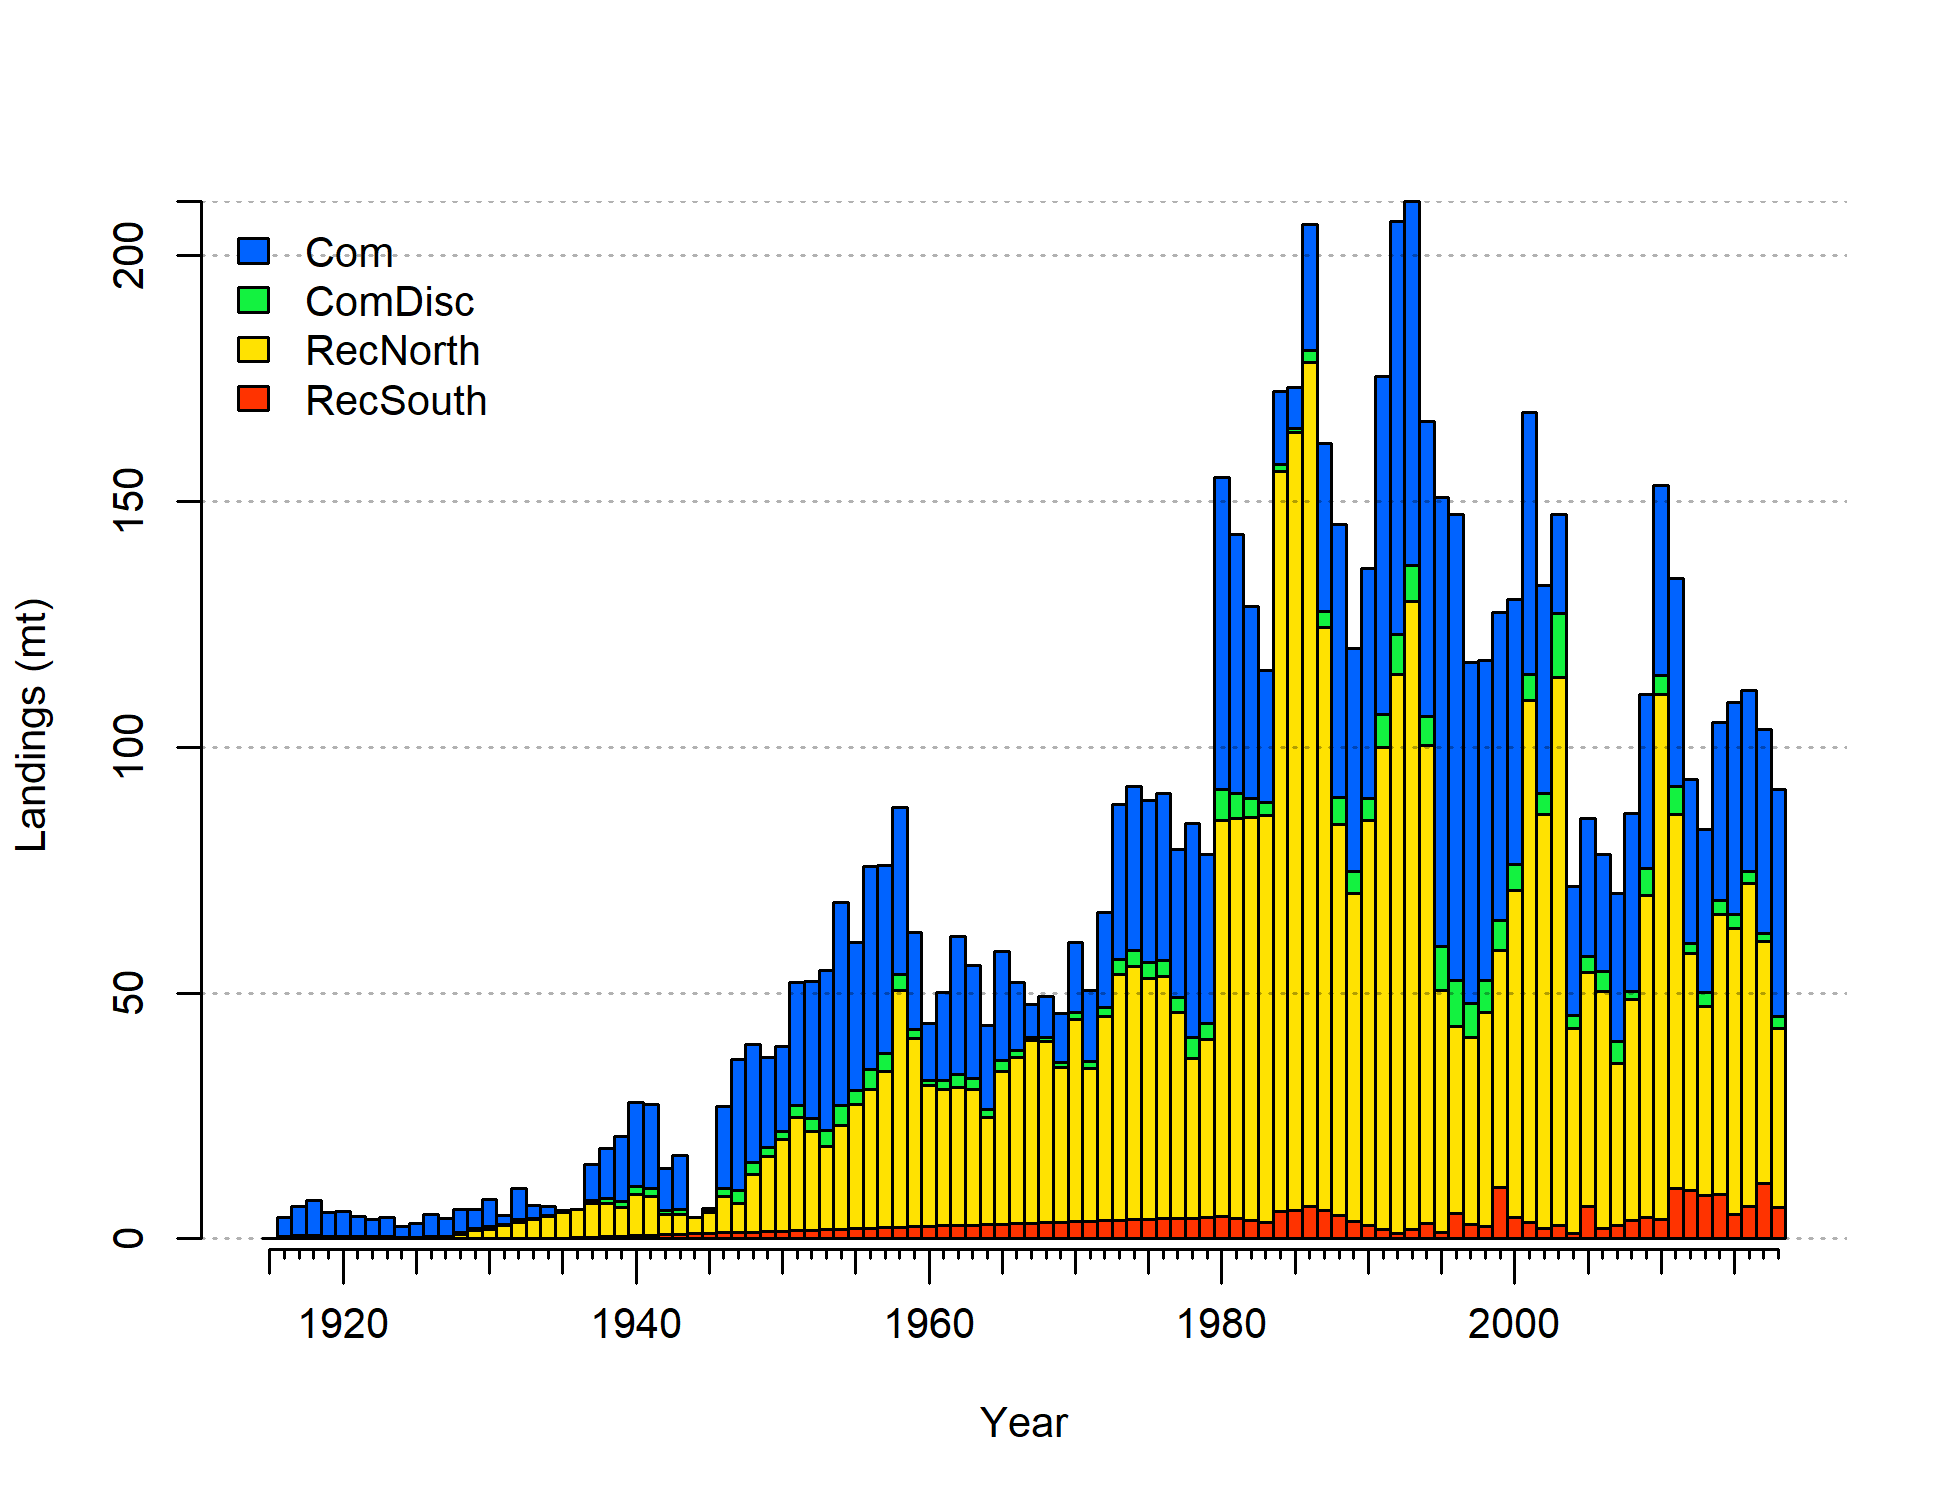
\includegraphics{r4ss/plots_mod1/catch2 landings stacked.png}
\caption{Catch history of GBY rockfish in the model.
\label{fig:r4ss_catches}}
\end{figure}

\begin{table}[ht]
\centering
\caption{Recent GBY rockfish landings (mt) by 
                                            fleet.} 
\label{tab:Exec_catch}
\begin{tabular}{l>{\centering}p{1in}>{\centering}p{1in}>{\centering}p{1in}>{\centering}p{.9in}>{\centering}p{.9in}>{\centering}p{.6in}}
  \hline
Year & Landings 1 & Landings 2 & Landings 3 & Landings 4 & Landings 5 & Total \\ 
  \hline
2005 & - & - & - & - & - & - \\ 
  2006 & - & - & - & - & - & - \\ 
  2007 & - & - & - & - & - & - \\ 
  2008 & - & - & - & - & - & - \\ 
  2009 & - & - & - & - & - & - \\ 
  2010 & - & - & - & - & - & - \\ 
  2011 & - & - & - & - & - & - \\ 
  2012 & - & - & - & - & - & - \\ 
  2013 & - & - & - & - & - & - \\ 
  2014 & - & - & - & - & - & - \\ 
   \hline
\end{tabular}
\end{table}

\FloatBarrier

\newpage

\subsection*{Data and Assessment}\label{data-and-assessment}
\addcontentsline{toc}{subsection}{Data and Assessment}

This a new full assessment for GBY rockfish, which was last assessed in
\ldots{} using Stock Synthesis Version xx. This assessment uses the
newest version of Stock Synthesis (3.30.xx). The model begins in 1916,
and assumes the stock was at an unfished equilibrium that year.

(Figure \ref{fig:assess_region_map}).

\begin{figure}
\centering
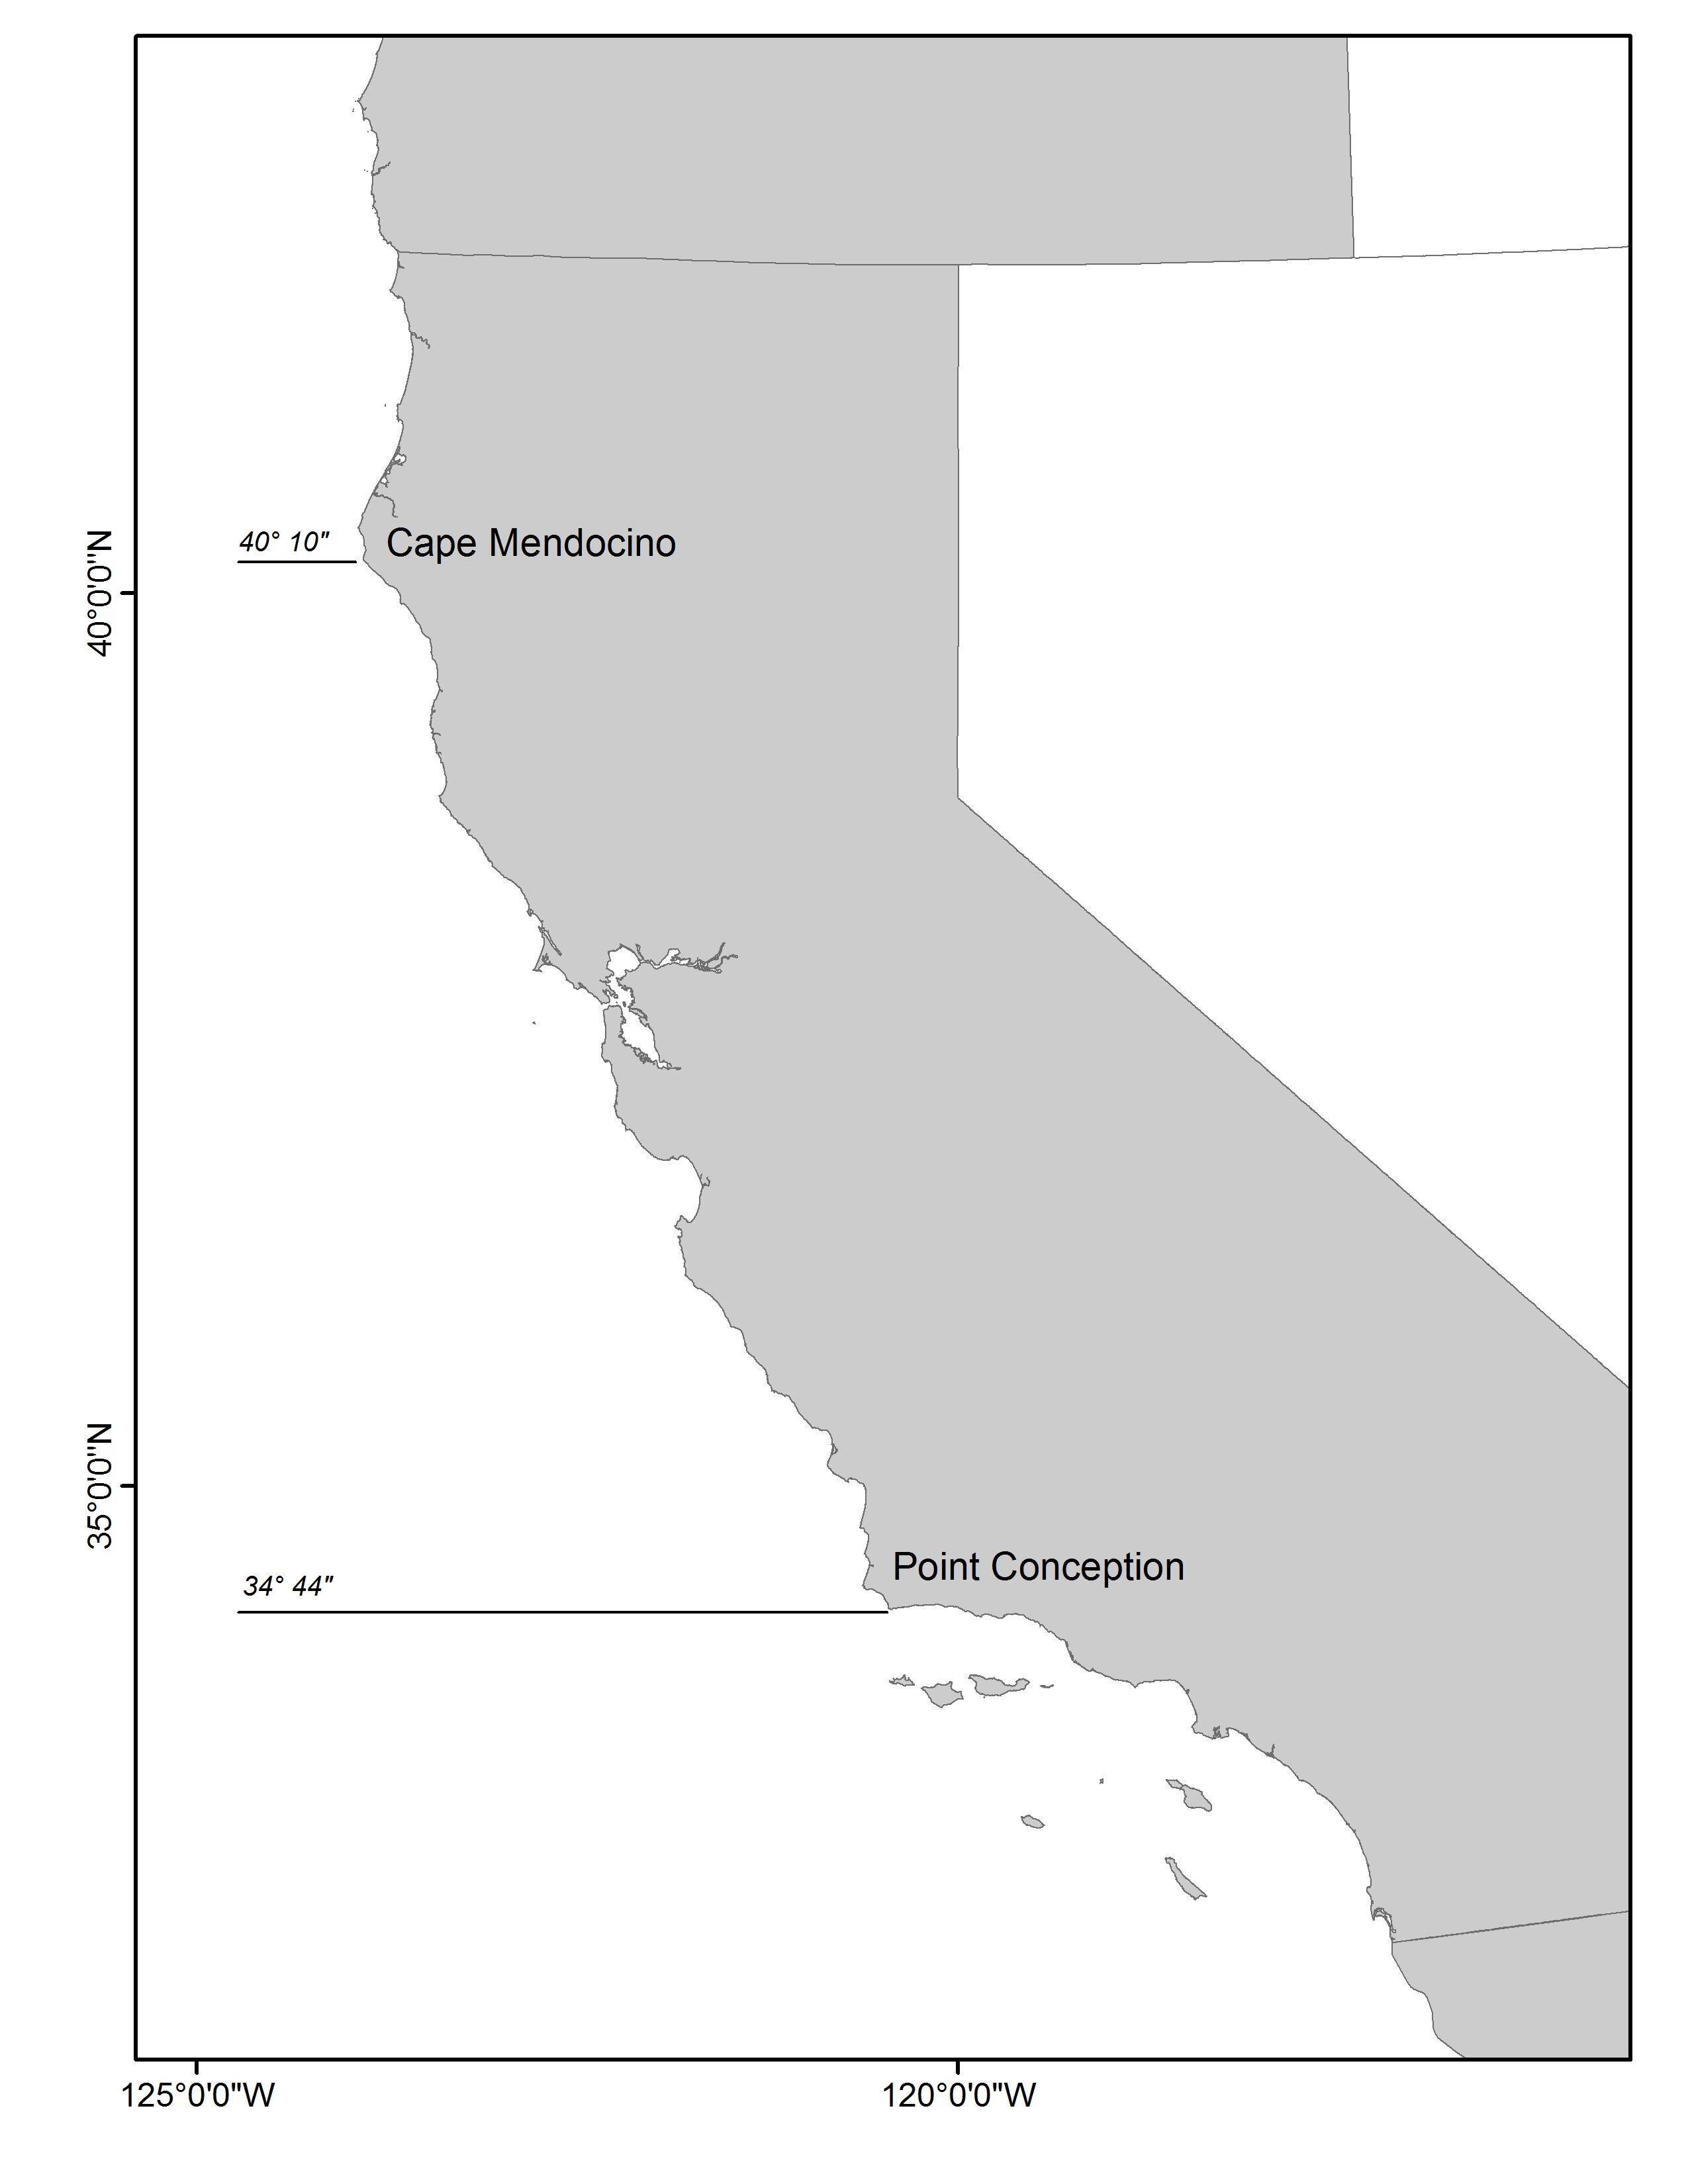
\includegraphics{Figures/assess_region_map.png}
\caption{Map depicting the distribution of California scorpionfish out
to 600 ft. The stock assessment is bounded at Pt. Conception in the
north to the U.S./Mexico border in the south.
\label{fig:assess_region_map}}
\end{figure}

\FloatBarrier

\subsection*{Stock Biomass}\label{stock-biomass}
\addcontentsline{toc}{subsection}{Stock Biomass}

(Figure \ref{fig:Spawnbio_all} and Table
\ref{tab:SpawningDeplete_mod1}).

The 2018 estimated spawning biomass relative to unfished equilibrium
spawning biomass is above the target of 40\% of unfished spawning
biomass at 45.1\% (95\% asymptotic interval: \(\pm\) 28.9\%-61.3\%)
(Figure \ref{fig:RelDeplete_all}). Approximate confidence intervals
based on the asymptotic variance estimates show that the uncertainty in
the estimated spawning biomass is high.

\FloatBarrier

\begin{table}[ht]
\centering
\caption{Recent trend in beginning of the 
                                      year spawning output and depletion for
                                      the model for GBY rockfish.} 
\label{tab:SpawningDeplete_mod1}
\begin{tabular}{l>{\centering}p{1.3in}>{\centering}p{1.2in}>{\centering}p{1in}>{\centering}p{1.2in}}
  \hline
Year & Spawning Output (million eggs) & \~{} 95\% confidence interval & Estimated depletion & \~{} 95\% confidence interval \\ 
  \hline
2010 & 864.575 & (604.3-1124.85) & 0.650 & (0.515-0.786) \\ 
  2011 & 795.859 & (549.68-1042.04) & 0.599 & (0.471-0.726) \\ 
  2012 & 741.221 & (507.57-974.88) & 0.558 & (0.437-0.678) \\ 
  2013 & 711.779 & (487.79-935.76) & 0.535 & (0.421-0.65) \\ 
  2014 & 691.107 & (474.44-907.77) & 0.520 & (0.41-0.63) \\ 
  2015 & 661.019 & (449.78-872.25) & 0.497 & (0.39-0.604) \\ 
  2016 & 634.707 & (425.9-843.51) & 0.477 & (0.371-0.584) \\ 
  2017 & 612.729 & (404.15-821.3) & 0.461 & (0.353-0.569) \\ 
  2018 & 599.056 & (389.03-809.08) & 0.451 & (0.34-0.561) \\ 
  2019 & 599.431 & (397.31-801.55) & 0.451 & (0.289-0.613) \\ 
   \hline
\end{tabular}
\end{table}

\FloatBarrier

\begin{figure}
\centering
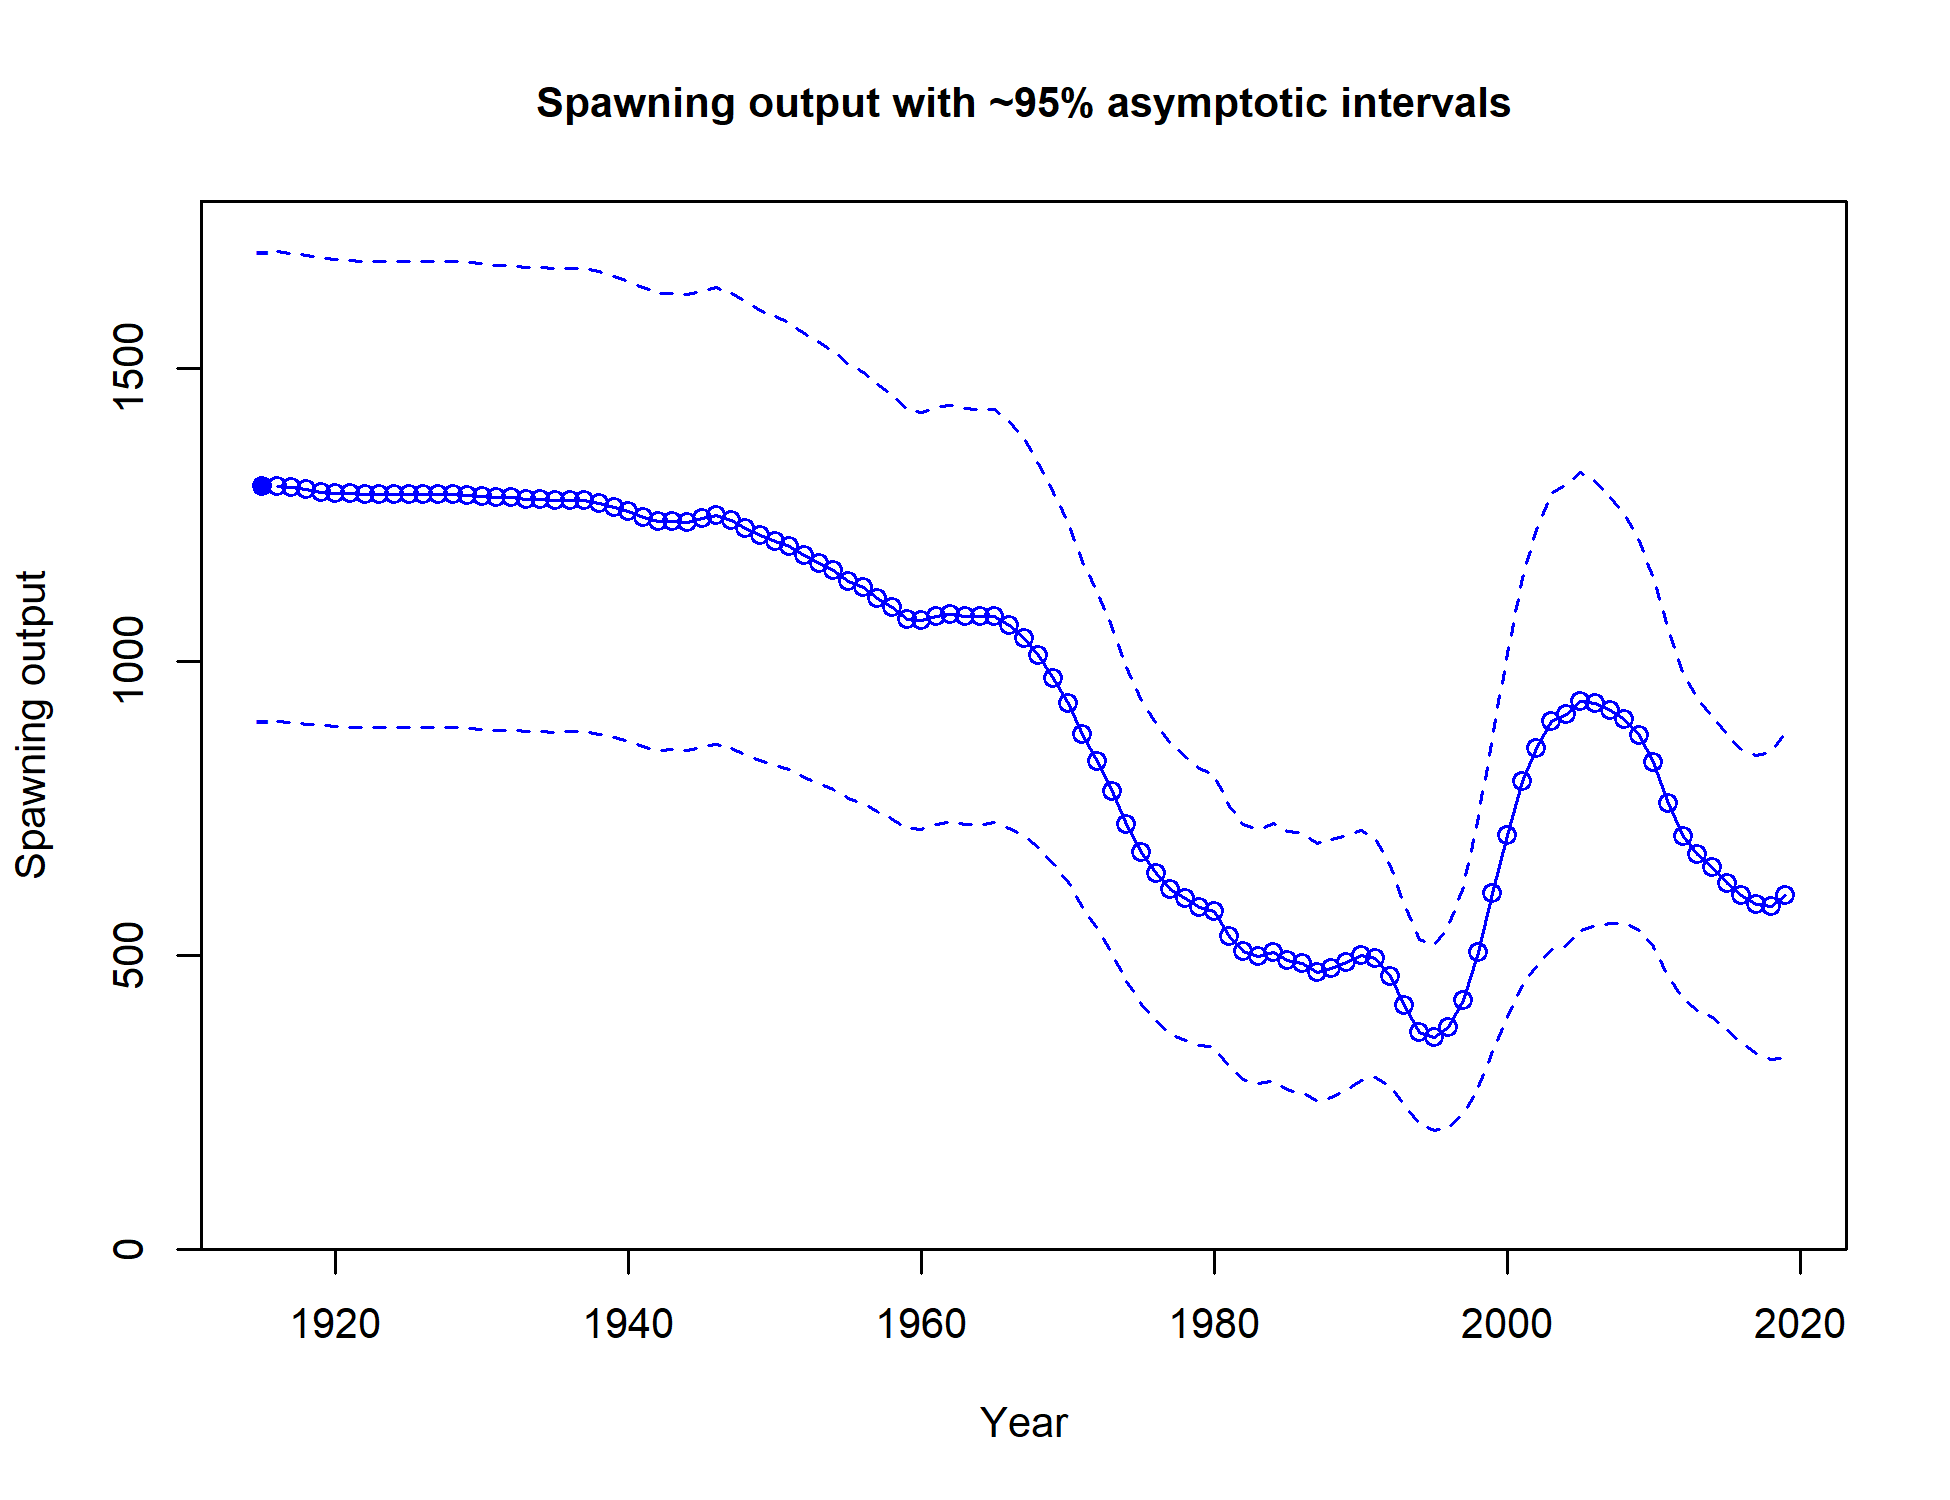
\includegraphics{r4ss/plots_mod1/ts7_Spawning_output_with_95_asymptotic_intervals_intervals.png}
\caption{Time series of spawning biomass trajectory (circles and line:
median; light broken lines: 95\% credibility intervals) for the base
case assessment model. \label{fig:Spawnbio_all}}
\end{figure}

\begin{figure}
\centering
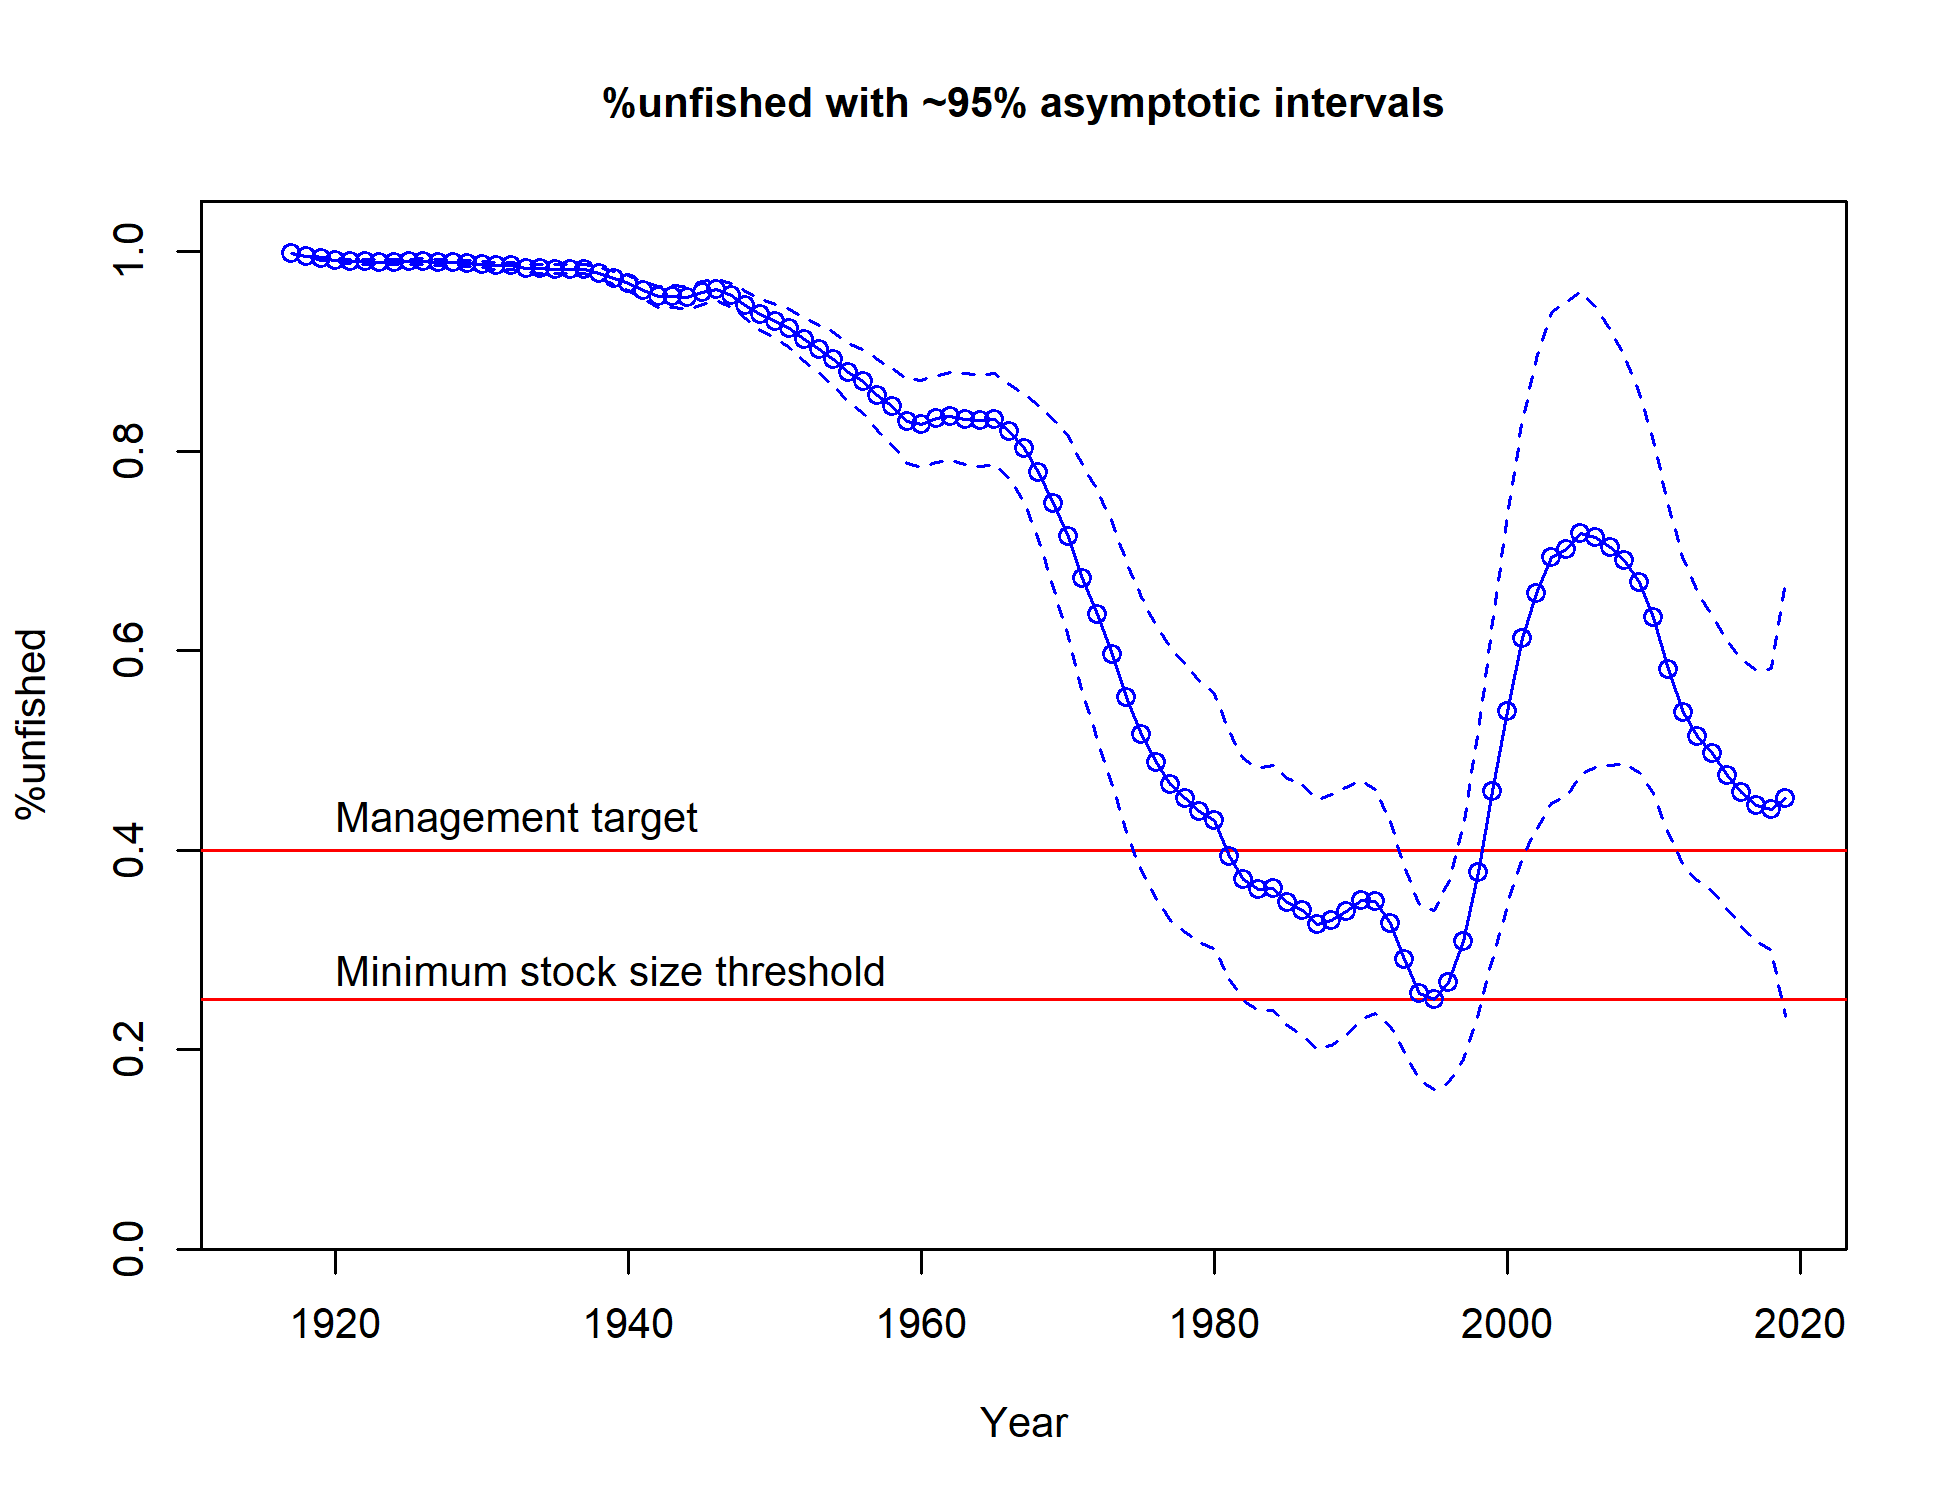
\includegraphics{r4ss/plots_mod1/ts9_unfished_with_95_asymptotic_intervals_intervals.png}
\caption{Estimated percent depletion with approximate 95\% asymptotic
confidence intervals (dashed lines) for the base case assessment model.
\label{fig:RelDeplete_all}}
\end{figure}

\FloatBarrier

\subsection*{Recruitment}\label{recruitment}
\addcontentsline{toc}{subsection}{Recruitment}

Recruitment deviations were estimated from xxxx-xxxx (Figure
\ref{fig:Recruits_all} and Table \ref{tab:Recruit_mod1}).

\begin{table}[ht]
\centering
\caption{Recent recruitment for the model.} 
\label{tab:Recruit_mod1}
\begin{tabular}{>{\centering}p{.8in}>{\centering}p{1.6in}>{\centering}p{1.3in}}
  \hline
Year & Estimated Recruitment (1,000s) & \~{} 95\% confidence interval \\ 
  \hline
2010 & 3218.83 & (1410.42 - 7345.97) \\ 
  2011 & 2746.99 & (1180.57 - 6391.77) \\ 
  2012 & 2631.66 & (1126.64 - 6147.16) \\ 
  2013 & 2767.28 & (1179.6 - 6491.88) \\ 
  2014 & 3916.77 & (1632.26 - 9398.66) \\ 
  2015 & 5510.34 & (2305.44 - 13170.55) \\ 
  2016 & 4079.14 & (1645.01 - 10115.07) \\ 
  2017 & 3360.32 & (1372 - 8230.16) \\ 
  2018 & 2968.86 & (1262.36 - 6982.25) \\ 
  2019 & 3352.25 & (1373.02 - 8184.58) \\ 
   \hline
\end{tabular}
\end{table}

\FloatBarrier

\begin{figure}
\centering
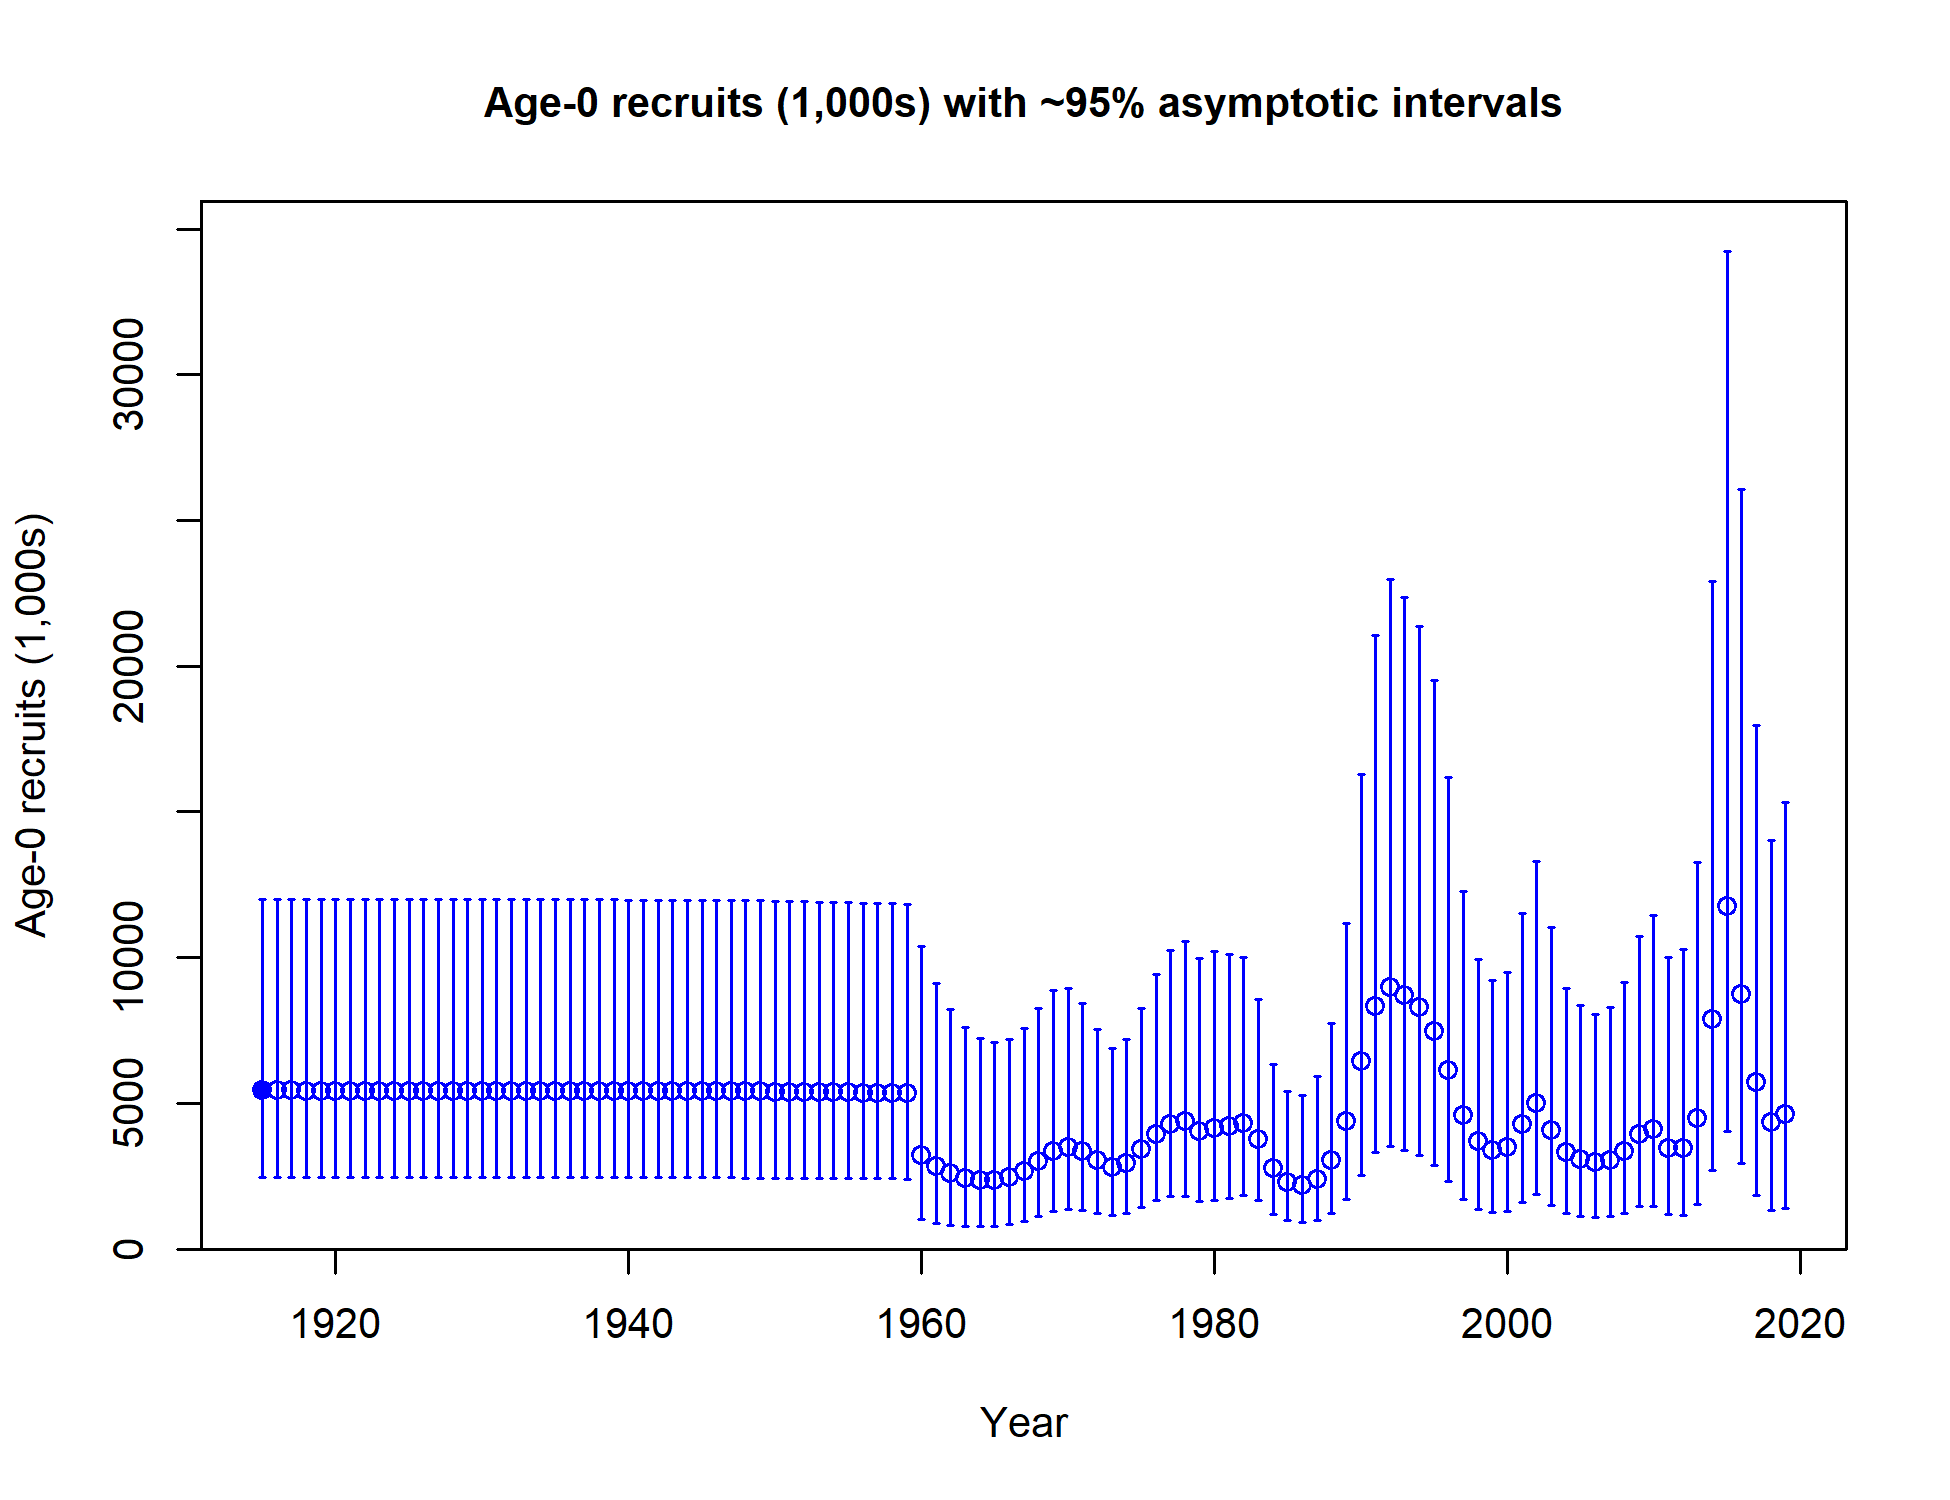
\includegraphics{r4ss/plots_mod1/ts11_Age-0_recruits_(1000s)_with_95_asymptotic_intervals.png}
\caption{Time series of estimated GBY rockfish recruitments for the
base-case model with 95\% confidence or credibility intervals.
\label{fig:Recruits_all}}
\end{figure}

\FloatBarrier

\subsection*{Exploitation status}\label{exploitation-status}
\addcontentsline{toc}{subsection}{Exploitation status}

Harvest rates estimated by the base model \ldots{}.. management target
levels (Table \ref{tab:SPR_Exploit_mod1} and Figure \ref{fig:SPR_all}).

\FloatBarrier

\begin{table}[ht]
\centering
\caption{Recent trend in spawning potential 
                                        ratio and exploitation for GBY rockfish in the model.  Fishing intensity is (1-SPR) 
                                        divided by 50\% (the SPR target) and exploitation 
                                        is F divided by F\textsubscript{SPR}.} 
\label{tab:SPR_Exploit_mod1}
\begin{tabular}{l>{\centering}p{1in}>{\centering}p{1.2in}>{\centering}p{1in}>{\centering}p{1.2in}}
  \hline
Year & Fishing intensity & \~{} 95\% confidence interval & Exploitation rate & \~{} 95\% confidence interval \\ 
  \hline
2009 & 0.67 & (0.49-0.85) & 0.08 & (0.06-0.1) \\ 
  2010 & 0.82 & (0.63-1.02) & 0.11 & (0.08-0.15) \\ 
  2011 & 0.81 & (0.61-1.01) & 0.11 & (0.08-0.14) \\ 
  2012 & 0.71 & (0.52-0.9) & 0.08 & (0.06-0.1) \\ 
  2013 & 0.67 & (0.49-0.86) & 0.07 & (0.05-0.09) \\ 
  2014 & 0.78 & (0.58-0.97) & 0.09 & (0.07-0.12) \\ 
  2015 & 0.81 & (0.61-1.01) & 0.10 & (0.07-0.13) \\ 
  2016 & 0.85 & (0.64-1.05) & 0.10 & (0.07-0.13) \\ 
  2017 & 0.85 & (0.64-1.06) & 0.10 & (0.06-0.13) \\ 
  2018 & 0.81 & (0.6-1.02) & 0.08 & (0.05-0.11) \\ 
   \hline
\end{tabular}
\end{table}

\FloatBarrier

\begin{figure}
\centering
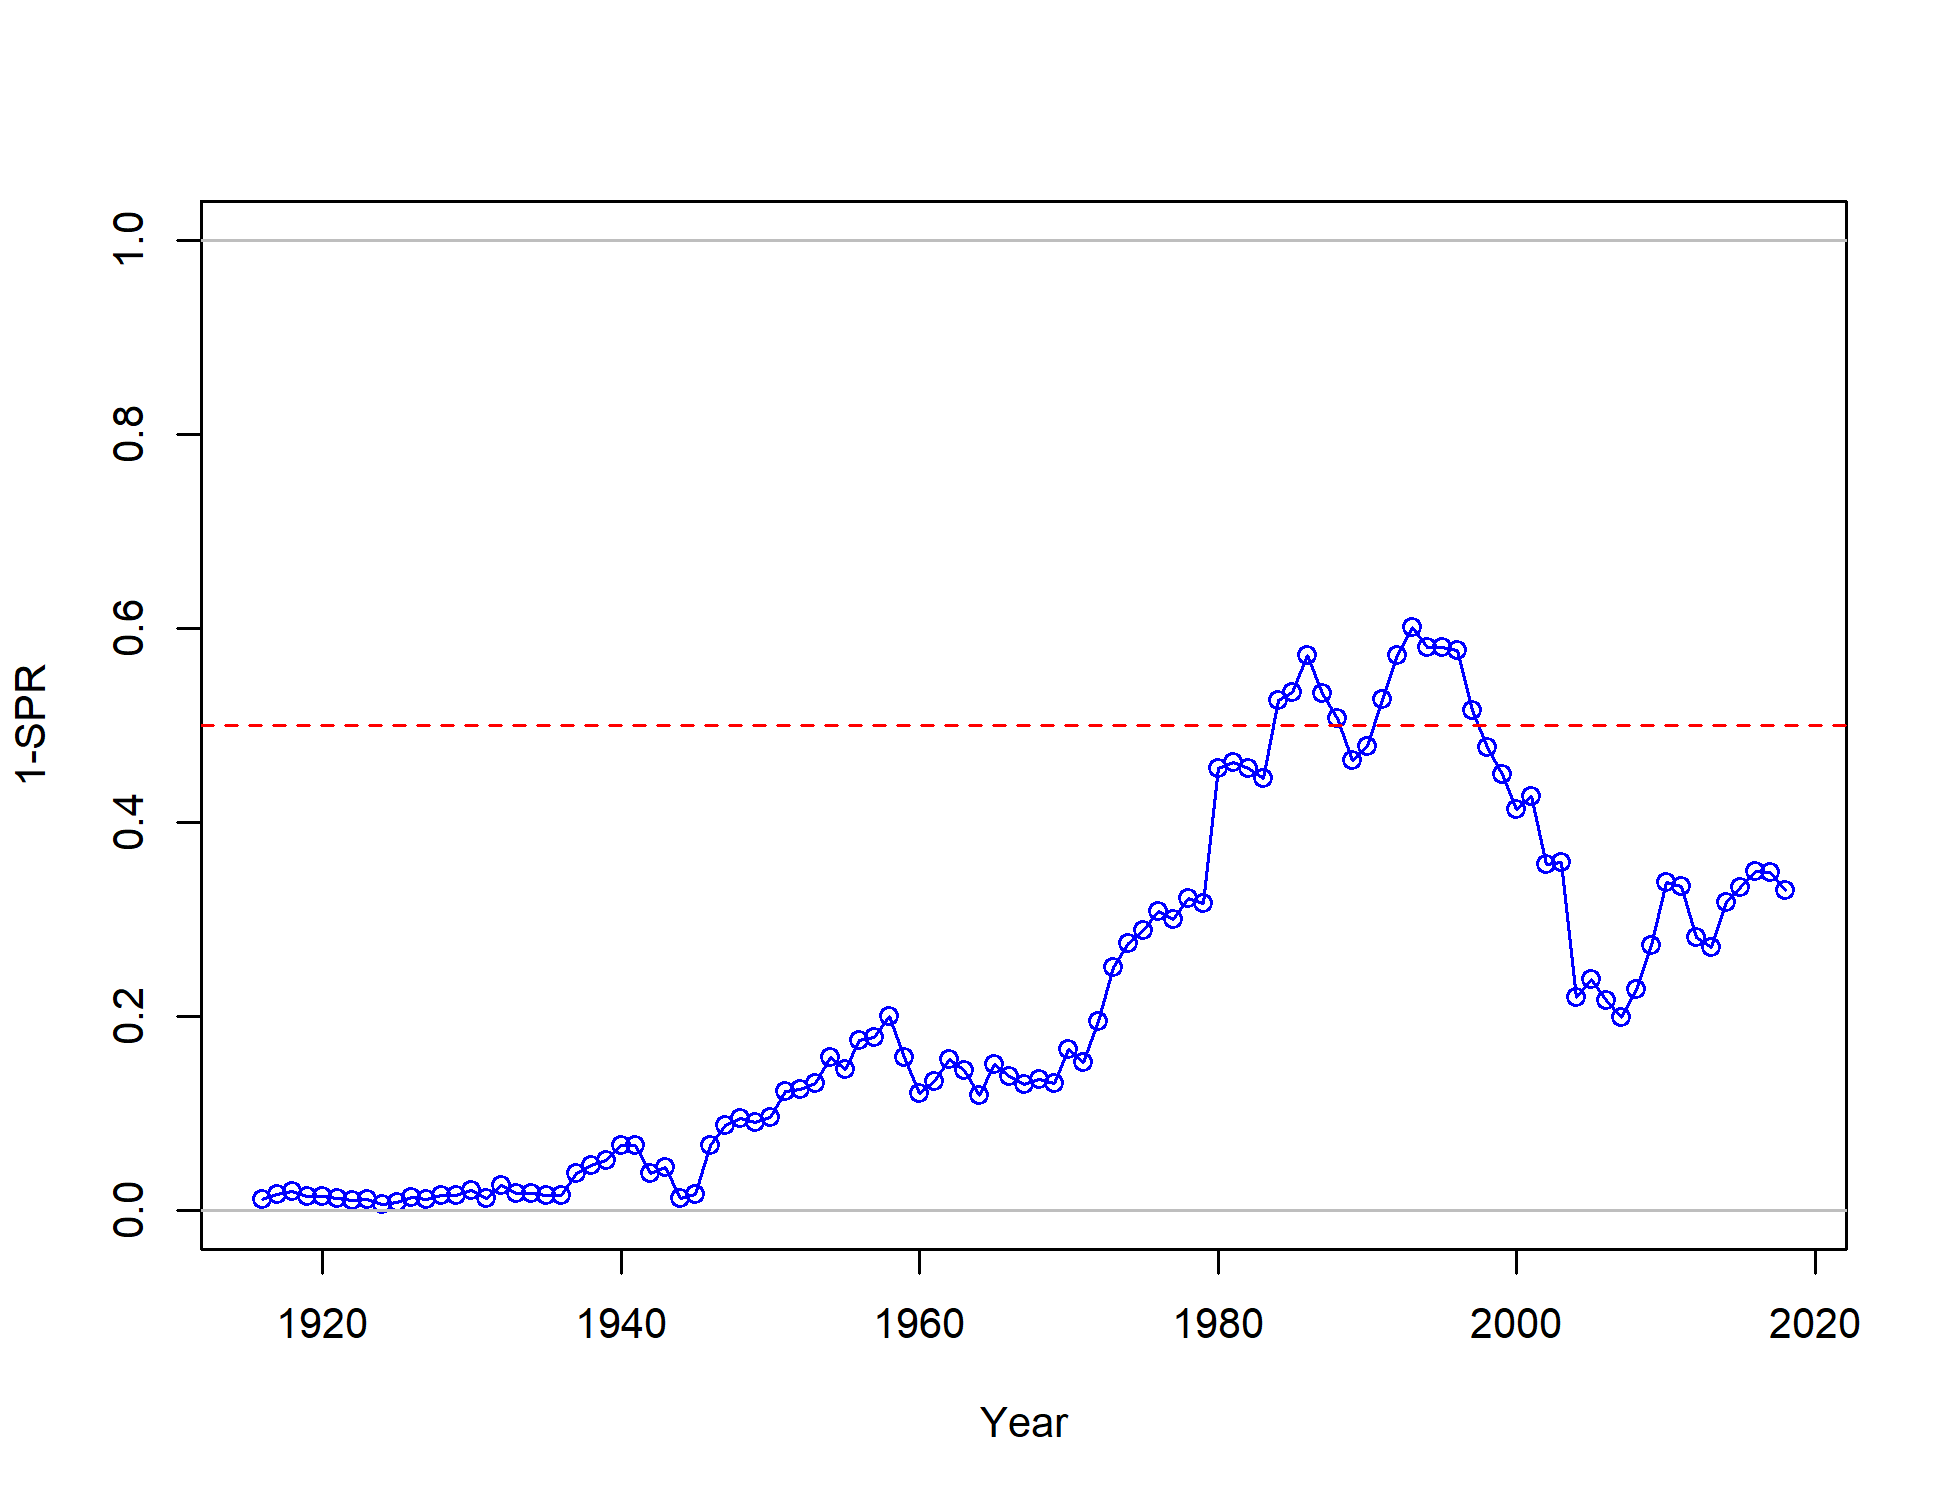
\includegraphics{r4ss/plots_mod1/SPR2_minusSPRseries.png}
\caption{Estimated spawning potential ratio (SPR) for the base-case
model. One minus SPR is plotted so that higher exploitation rates occur
on the upper portion of the y-axis. The management target is plotted as
a red horizontal line and values above this reflect harvests in excess
of the overfishing proxy based on the SPR\textsubscript{50\%} harvest
rate. The last year in the time series is 2018. \label{fig:SPR_all}}
\end{figure}

\FloatBarrier

\subsection*{Ecosystem Considerations}\label{ecosystem-considerations}
\addcontentsline{toc}{subsection}{Ecosystem Considerations}

In this assessment, ecosystem considerations were not explicitly
included in the analysis.\\
This is primarily due to a lack of relevant data and results of analyses
(conducted elsewhere) that could contribute ecosystem-related
quantitative information for the assessment.

\subsection*{Reference Points}\label{reference-points}
\addcontentsline{toc}{subsection}{Reference Points}

This stock assessment estimates that GBY rockfish in the model is above
the biomass target (\(SB_{40\%}\)), and well above the minimum stock
size threshold (\(SB_{25\%}\)). The estimated relative depletion level
for the base model in 2019 is 45.1\% (95\% asymptotic interval: \(\pm\)
28.9\%-61.3\%, corresponding to an unfished spawning biomass of 599.431
million eggs (95\% asymptotic interval: 397.31-801.55 million eggs) of
spawning biomass in the base model (Table \ref{tab:Ref_pts_mod1}).
Unfished age 1+ biomass was estimated to be 1,969 mt in the base case
model. The target spawning biomass (\(SB_{40\%}\)) is 532 million eggs,
which corresponds with an equilibrium yield of 145 mt. Equilibrium yield
at the proxy \(F_{MSY}\) harvest rate corresponding to \(SPR_{50\%}\) is
136 mt (Figure \ref{fig:Yield_all}).

\FloatBarrier

\begin{table}[ht]
\centering
\caption{Summary of reference 
                                      points and management quantities for the 
                                      base case model.} 
\label{tab:Ref_pts_mod1}
\begin{tabular}{>{\raggedright}p{4.1in}>{\raggedleft}p{.62in}>{\raggedleft}p{.62in}>{\raggedleft}p{.62in}}
  \hline
\textbf{Quantity} & \textbf{Estimate} & \textbf{Low 2.5\%  limit} & \textbf{High 2.5\%  limit} \\ 
  \hline
Unfished spawning output (million eggs) & 1,329 & 1,030 & 1,629 \\ 
  Unfished age 1+ biomass (mt) & 1,969 & 1,642 & 2,296 \\ 
  Unfished recruitment ($R_{0}$) & 3,749 & 1,561 & 5,937 \\ 
  Spawning output(2018 million eggs) & 599 & 389 & 809 \\ 
  Depletion (2018) & 0.451 & 0.34 & 0.561 \\ 
  \textbf{$\text{Reference points based on } \mathbf{SB_{40\%}}$} &  &  &  \\ 
  Proxy spawning output ($B_{40\%}$) & 532 & 456 & 607 \\ 
  SPR resulting in $B_{40\%}$ ($SPR_{B40\%}$) & 0.458 & 0.458 & 0.458 \\ 
  Exploitation rate resulting in $B_{40\%}$ & 0.139 & 0.107 & 0.171 \\ 
  Yield with $SPR_{B40\%}$ at $B_{40\%}$ (mt) & 145 & 105 & 184 \\ 
  \textbf{\textit{Reference points based on SPR proxy for MSY}} &  &  &  \\ 
  Spawning output & 593 & 509 & 677 \\ 
  $SPR_{proxy}$ & 0.5 &  &  \\ 
  Exploitation rate corresponding to $SPR_{proxy}$ & 0.121 & 0.093 & 0.15 \\ 
  Yield with $SPR_{proxy}$ at $SB_{SPR}$ (mt) & 136 & 99 & 173 \\ 
  \textbf{\textit{Reference points based on estimated MSY values}} &  &  &  \\ 
  Spawning output at $MSY$ ($SB_{MSY}$) & 297 & 248 & 346 \\ 
  $SPR_{MSY}$ & 0.299 & 0.288 & 0.31 \\ 
  Exploitation rate at $MSY$ & 0.234 & 0.171 & 0.296 \\ 
  Dead Catch $MSY$ (mt) & 165 & 117 & 212 \\ 
  Retained Catch $MSY$ (mt) & 165 & 117 & 212 \\ 
   \hline
\end{tabular}
\end{table}

\FloatBarrier

\subsection*{Management Performance}\label{management-performance}
\addcontentsline{toc}{subsection}{Management Performance}

Table \ref{tab:mnmgt_perform}

\begin{table}[ht]
\centering
\caption{Recent trend in total catch and commercial 
                              landings (mt) relative to the management guidelines. 
                              Estimated total catch reflect the commercial landings 
                              plus the model estimated discarded biomass.} 
\label{tab:mnmgt_perform}
\scalebox{0.9}{
\begin{tabular}{>{\raggedleft}p{1in}>{\centering}p{1in}>{\centering}p{1in}>{\centering}p{1in}>{\centering}p{1in}}
  \hline
Year & OFL (mt; ABC prior to 2011) & ABC (mt) & ACL (mt; OY prior to 2011) & Estimated total catch (mt) \\ 
  \hline
\textbf{2007} & - & - & - & - \\ 
  \textbf{2008} & - & - & - & - \\ 
  \textbf{2009} & - & - & - & - \\ 
  \textbf{2010} & - & - & - & - \\ 
  \textbf{2011} & - & - & - & - \\ 
  \textbf{2012} & - & - & - & - \\ 
  \textbf{2013} & - & - & - & - \\ 
  \textbf{2014} & - & - & - & - \\ 
  \textbf{2015} & - & - & - & - \\ 
  \textbf{2016} & - & - & - & - \\ 
  \textbf{2017} & - & - & - & - \\ 
  \textbf{2018} & - & - & - & - \\ 
   \hline
\end{tabular}
}
\end{table}

\subsection*{Unresolved Problems and Major
Uncertainties}\label{unresolved-problems-and-major-uncertainties}
\addcontentsline{toc}{subsection}{Unresolved Problems and Major
Uncertainties}

\FloatBarrier

\subsection*{Decision Table}\label{decision-table}
\addcontentsline{toc}{subsection}{Decision Table}

\begin{table}[ht]
\centering
\caption{Projections of potential OFL (mt) for 
                                        each model, using the base model forecast.} 
\label{tab:OFL_projection}
\begin{tabular}{lr}
  \hline
Year & OFL \\ 
  \hline
2019 & 145.83 \\ 
   \hline
\end{tabular}
\end{table}\begin{table}[ht]
\centering
\caption{Summary of 10-year 
                                             projections beginning in 2020 
                                             for alternate states of nature based on 
                                             an axis of uncertainty for the model.  Columns range over low, mid, and high
                                             states of nature, and rows range over different 
                                             assumptions of catch levels. An entry of "--" 
                                             indicates that the stock is driven to very low 
                                             abundance under the particular scenario.} 
\label{tab:Decision_table_mod1}
\scalebox{0.85}{
\begin{tabular}{l|cc|>{\centering}p{.7in}c|>{\centering}p{.7in}c|>{\centering}p{.7in}c}
   \multicolumn{3}{c}{}  &  \multicolumn{2}{c}{} 
                               & \multicolumn{2}{c}{\textbf{States of nature}} 
                               & \multicolumn{2}{c}{} \\
  \multicolumn{3}{c}{}  &  \multicolumn{2}{c}{Low M 0.05} 
                               & \multicolumn{2}{c}{Base M 0.07} 
                               &  \multicolumn{2}{c}{High M 0.09} \\
 \hline
 & Year & Catch & Spawning Output & Depletion & Spawning Output & Depletion & Spawning Output & Depletion \\ 
  \hline
 & 2019 & - & - & - & - & - & - & - \\ 
   & 2020 & - & - & - & - & - & - & - \\ 
   & 2021 & - & - & - & - & - & - & - \\ 
  40-10 Rule,  & 2022 & - & - & - & - & - & - & - \\ 
  Low M & 2023 & - & - & - & - & - & - & - \\ 
   & 2024 & - & - & - & - & - & - & - \\ 
   & 2025 & - & - & - & - & - & - & - \\ 
   & 2026 & - & - & - & - & - & - & - \\ 
   & 2027 & - & - & - & - & - & - & - \\ 
   & 2028 & - & - & - & - & - & - & - \\ 
   \hline
 & 2019 & - & - & - & - & - & - & - \\ 
   & 2020 & - & - & - & - & - & - & - \\ 
   & 2021 & - & - & - & - & - & - & - \\ 
  40-10 Rule & 2022 & - & - & - & - & - & - & - \\ 
   & 2023 & - & - & - & - & - & - & - \\ 
   & 2024 & - & - & - & - & - & - & - \\ 
   & 2025 & - & - & - & - & - & - & - \\ 
   & 2026 & - & - & - & - & - & - & - \\ 
   & 2027 & - & - & - & - & - & - & - \\ 
   & 2028 & - & - & - & - & - & - & - \\ 
   \hline
 & 2019 & - & - & - & - & - & - & - \\ 
   & 2020 & - & - & - & - & - & - & - \\ 
   & 2021 & - & - & - & - & - & - & - \\ 
  40-10 Rule, & 2022 & - & - & - & - & - & - & - \\ 
  High M & 2023 & - & - & - & - & - & - & - \\ 
   & 2024 & - & - & - & - & - & - & - \\ 
   & 2025 & - & - & - & - & - & - & - \\ 
   & 2026 & - & - & - & - & - & - & - \\ 
   & 2027 & - & - & - & - & - & - & - \\ 
   & 2028 & - & - & - & - & - & - & - \\ 
   \hline
 & 2019 & - & - & - & - & - & - & - \\ 
   & 2020 & - & - & - & - & - & - & - \\ 
   & 2021 & - & - & - & - & - & - & - \\ 
  Average & 2022 & - & - & - & - & - & - & - \\ 
  Catch & 2023 & - & - & - & - & - & - & - \\ 
   & 2024 & - & - & - & - & - & - & - \\ 
   & 2025 & - & - & - & - & - & - & - \\ 
   & 2026 & - & - & - & - & - & - & - \\ 
   & 2027 & - & - & - & - & - & - & - \\ 
   & 2028 & - & - & - & - & - & - & - \\ 
   \hline
\end{tabular}
}
\end{table}

\begin{sidewaystable}[ht]
\centering
\caption{Base case results summary.} 
\label{tab:base_summary}
\scalebox{0.6}{
\begin{tabular}{r>{\centering}p{1.1in}>{\centering}p{1.1in}>{\centering}p{1.1in}>{\centering}p{1.1in}>{\centering}p{1.1in}>{\centering}p{1.1in}>{\centering}p{1.1in}>{\centering}p{1.1in}>{\centering}p{1.1in}>{\centering}p{1.1in}}
  \hline
Quantity & 2010 & 2011 & 2012 & 2013 & 2014 & 2015 & 2016 & 2017 & 2018 & 2019 \\ 
  \hline
Landings (mt) &  &  &  &  &  &  &  &  &  &  \\ 
  Total Est. Catch (mt) &  &  &  &  &  &  &  &  &  &  \\ 
  OFL (mt) &  &  &  &  &  &  &  &  &  &  \\ 
  ACL (mt) &  &  &  &  &  &  &  &  &  &  \\ 
   \hline
(1-$SPR$)(1-$SPR_{50\%}$) & 0.82 & 0.81 & 0.71 & 0.67 & 0.78 & 0.81 & 0.85 & 0.85 & 0.81 &  \\ 
   \hline
Exploitation rate & 0.11 & 0.11 & 0.08 & 0.07 & 0.09 & 0.10 & 0.10 & 0.10 & 0.08 &  \\ 
  Age 1+ biomass (mt) & 1391.63 & 1332.20 & 1246.97 & 1184.00 & 1156.13 & 1140.65 & 1116.13 & 1101.05 & 1097.89 & 1118.10 \\ 
   \hline
Spawning Output & 864.6 & 795.9 & 741.2 & 711.8 & 691.1 & 661.0 & 634.7 & 612.7 & 599.1 & 599.4 \\ 
  ~95\% CI & (604.3-1124.85) & (549.68-1042.04) & (507.57-974.88) & (487.79-935.76) & (474.44-907.77) & (449.78-872.25) & (425.9-843.51) & (404.15-821.3) & (389.03-809.08) & (397.31-801.55) \\ 
   \hline
Depletion & 0.7 & 0.6 & 0.6 & 0.5 & 0.5 & 0.5 & 0.5 & 0.5 & 0.5 & 0.5 \\ 
  ~95\% CI & (0.515-0.786) & (0.471-0.726) & (0.437-0.678) & (0.421-0.65) & (0.41-0.63) & (0.39-0.604) & (0.371-0.584) & (0.353-0.569) & (0.34-0.561) & (0.289-0.613) \\ 
   \hline
Recruits & 3218.83 & 2746.99 & 2631.66 & 2767.28 & 3916.77 & 5510.34 & 4079.14 & 3360.32 & 2968.86 & 3352.25 \\ 
  ~95\% CI & (1410.42 - 7345.97) & (1180.57 - 6391.77) & (1126.64 - 6147.16) & (1179.6 - 6491.88) & (1632.26 - 9398.66) & (2305.44 - 13170.55) & (1645.01 - 10115.07) & (1372 - 8230.16) & (1262.36 - 6982.25) & (1373.02 - 8184.58) \\ 
   \hline
\end{tabular}
}
\end{sidewaystable}

\begin{figure}
\centering
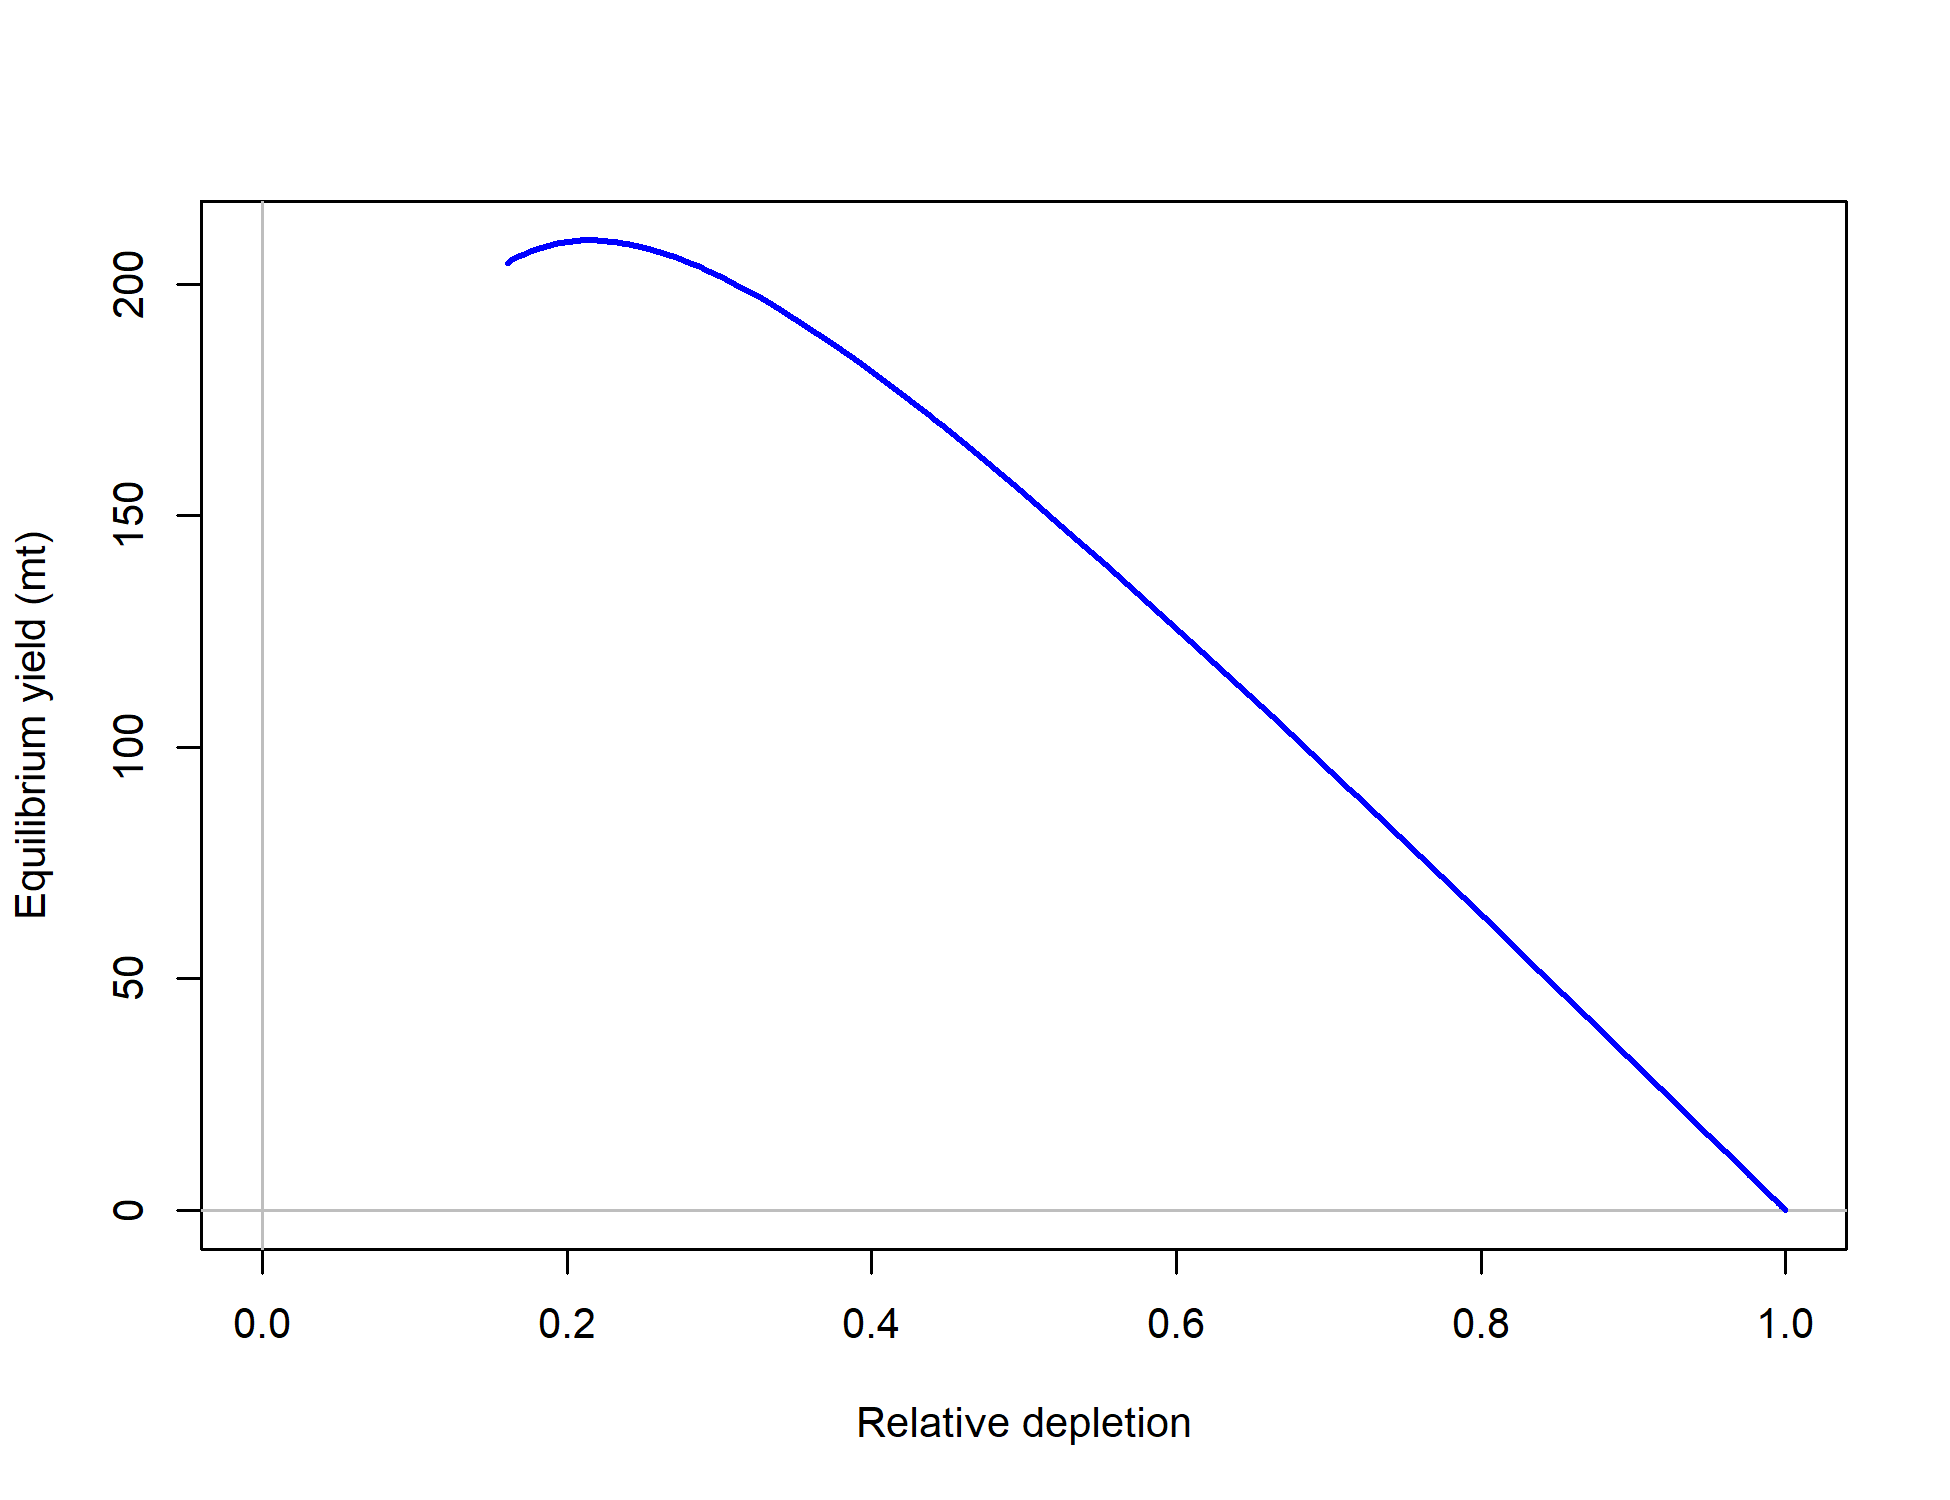
\includegraphics{r4ss/plots_mod1/yield1_yield_curve.png}
\caption{Equilibrium yield curve for the base case model. Values are
based on the 2018 fishery selectivity and with steepness fixed at 0.718.
\label{fig:Yield_all}}
\end{figure}

\FloatBarrier

\newpage

\subsection*{Research and Data Needs}\label{research-and-data-needs}
\addcontentsline{toc}{subsection}{Research and Data Needs}

We recommend the following research be conducted before the next
assessment:

\begin{enumerate}

\item \textbf{xxxx}: 

\item \textbf{xxxx}:

\item \textbf{xxxx}:

\item \textbf{xxxx}:

\item \textbf{xxxx}:

\end{enumerate}

\FloatBarrier

\newpage

\renewcommand{\thefigure}{\arabic{figure}}
\renewcommand{\thetable}{\arabic{table}}

\setcounter{figure}{0} \setcounter{table}{0}

\pagenumbering{arabic}

\section{Introduction}\label{introduction}

\subsection{Basic Information and Life
History}\label{basic-information-and-life-history}

\subsection{Early Life History}\label{early-life-history}

\subsection{Map}\label{map}

A map showing the scope of the assessment and depicting boundaries for
fisheries or data collection strata is provided in Figure
\ref{fig:boundary_map}.

\subsection{Ecosystem Considerations}\label{ecosystem-considerations-1}

In this assessment, ecosystem considerations were not explicitly
included in the analysis. This is primarily due to a lack of relevant
data and results of analyses (conducted elsewhere) that could contribute
ecosystem-related quantitative information for the assessment.

\subsection{Fishery Information}\label{fishery-information}

\subsection{Summary of Management
History}\label{summary-of-management-history}

\subsection{Management Performance}\label{management-performance-1}

Table \ref{tab:mnmgt_perform}

\subsection{Fisheries Off Mexico or
Canada}\label{fisheries-off-mexico-or-canada}

\section{Assessment}\label{assessment}

\subsection{Data}\label{data}

Data used in the GBY rockfish assessment are summarized in Figure
\ref{fig:data_plot}. Descriptions of the data sources are in the
following sections.

\subsubsection{Commercial Fishery
Landings}\label{commercial-fishery-landings}

Commercial landings in California are based on two primary data sources:
a cooperative port sampling program (California Cooperative Groundfish
Survey, \href{https://calcom.psmfc.org/}{CALCOM}) that collects
information including species composition data (i.e.~the proportion of
species landed in a sampling stratum), and landing receipts (sometimes
called ``fish tickets'') that are a record of pounds landed in a given
stratum. Strata in California are defined by market category, year,
quarter, gear group, port complex, and disposition (live or dead).
Although many market categories are named after actual species, catch in
a given market category can consist of several species. All landings
used in this assessment are ``expanded'' landings, i.e., species
composition data collected by port samplers were used to allocate pounds
recorded on landing receipts to species. Use of the ``Gopher Rockfish''
or the ``Black-and-Yellow Rockfish'' categories alone to represent
actual landings of GBY would not be accurate. See Pearson et al.
Appendix C (\protect\hyperlink{ref-Pearson2008}{2008}) for a simple
example of the expansion calculations. Data from the California
Cooperative Groundfish Survey, species compositions, and expanded
landings estimates are stored in the CALCOM database at the Pacific
States Marine Fisheries Commission, a central repository of commercial
landings data for the U.S. West Coast.

Commercial catches of black-and-yellow rockfish from 1916-1968 and for
gopher rockfish from 1937-1968 were queried (4 April 2019) from the
California Catch Reconstruction (Ralston et al.
\protect\hyperlink{ref-Ralston2010}{2010}). Landings in this database
are divided into trawl and `non-trawl.' Since the majority of GBYR are
caught in the commercial fixed gear fisheries, only estimated catch in
the `non-trawl' was used. A total of 0.154 mt (3.18\%) were removed from
Eureka commercial landings (based on current proportions of commercial
catch from north of Cape Mencodino in Eureka) since the assessment
represents the GBYR stock south of Cape Mendocino.

Commercial landings from 1969-2018 were queried for a final time from
the CALCOM database on 4 April 2019 (Table \ref{tab:commCatches}.
Commercial landings were also queried from PacFIN (Pacific Fisheries
Inforamtion Network) for a final time on 3 June 2019 for comparison to
CALCOM landings. There are very small differences in commercial landings
between CALCOM and PacFIN from 1981-2018 (Figure
\ref:fig:Calcom\_vs\_Pacfin\}). Landings estiamtes from CALCOM were used
in the assessment. Landings were stratified by year, quarter, live/dead,
market category, gear group, port complex, and source of species
composition data (actual port samples, borrowed samples, or assumed
nominal market category). Data from individual quarters were aggregated
at the year level. Fish landed live or dead were combined, due to
changes over time in the reliability of condition information (D.
Pearson, pers. comm.). From 1916-1968, on average, 74\% of GBYR were
landed north of Point Conception, which rose to 97\% from 1978-2018.
Given the smaller landings south of Point Conception and the similar
length composition of GBYR north and south of Pt. Conception, no spatial
separation was considered for the commercial fleet.

\subsubsection{Commercial Discards}\label{commercial-discards}

The West Coast Groundfish Observer Program (WCGOP) provides observer
data on discarding practices across sectors back to 2003. Gopher and
black-and-yellow rockfishes have different depth-stratified commercial
fishery discard mortality rates (Pacific Fishery Managment Council
\protect\hyperlink{ref-PSMFC2018}{2018}). In consultation with WCGOP
staff, the STAT used estimates of total discard mortality from WCGOP's
Groundfish Expanded Mortality Multiyear (GEMM) report. WCGOP observes
between 1-5\% of nearshore fixed gear landings annually south of
\(40^\circ 10^\prime\) N. latitude (coverage rates available
\href{https://www.nwfsc.noaa.gov/research/divisions/fram/observation/data_products/sector_products.cfm\#ob}{here}).
The expanded estimates of total discard by species is calculated as the
ratio of the discard of the individual species observed by WCGOP divided
by the observed landings from PacFIN landing receipts. WCGOP discard
estimates for the nearshore fixed gear fishery take into account the
depth distribution of landings in order to appropriately apply the
depth-stratified discard mortality rates by species (Somers, K.A., J.
Jannot, V. Tuttle, K. Richerson and McVeigh
\protect\hyperlink{ref-Somers2018}{2018}). The discard mortality for
2018 was estimated as an average of the discard mortality from
20213-2017. Discard mortality was estimated from the period prior to
WCGOP discard estimates (1916-2002) based on the average discard
mortality rate from 2003-2016 (2017 was excluded because 2017 discard
mortality was disproportionately higher than all other years) (Table
\ref{tab:CommCatches}).

\subsubsection{Commercial Fishery Length and Age
Data}\label{commercial-fishery-length-and-age-data}

The input sample sizes were calculated via the Stewart Method (Ian
Stewart, personal communication, IPHC):

\begin{centering}

Input effN = $N_{\text{trips}} + 0.138 * N_{\text{fish}}$ if $N_{\text{fish}}/N_{\text{trips}}$ is $<$ 44

Input effN = $7.06 * N_{\text{trips}}$ if $N_{\text{fish}}/N_{\text{trips}}$ is $\geq$ 44

\end{centering}

\subsubsection{Sport Fishery Removals and
Discards}\label{sport-fishery-removals-and-discards}

Three data sources were used to estimate retained and discard mortality
for the recreational fishing fleet; the California Catch Reconstruction
(Ralston et al. \protect\hyperlink{ref-Ralston2010}{2010}) and the
California Department of Fish and Wildlife MRFSS (1980-2003) and CRFS
(2004-2018) databases.

\emph{Historical recreational landings and discard, 1928-1980} Ralston
et al. (\protect\hyperlink{ref-Ralston2010}{2010}) reconstructed
estimates of recreational rockfish catch and discard in California,
1928-1980. Reported landings of total rockfish were allocated to species
based on several sources of species composition data. Estimates of GBYR
landings and discard (combined) from 1928-1979 are available from the
SWFSC. For this assessment, historical recreational catch was stratified
by year and area (north and south of Point Conception). The catches of
GBYR reported in Ralston et al.
(\protect\hyperlink{ref-Ralston2010}{2010}) are higher than expected
given the more recent catches of GBYR south of Pt. Conception and the
species' ranges (Figure \ref{fig:Catches_original}). The California
Catch Reconstruction used a linear from from 1928-1936 that was not
altered. From 1937-1979 linear ramp to the average recreational landing
from 1980 and 1983 (1981-1982 catches interpolated as described in the
next section) of 4.3 mt. The recreational catches north of Pt.
Conception were not altered from the original catch reconstruction. The
resulting alternate recreational catch streams are in (Table
\ref{tab:Rec_removal} and Figure \ref{fig:Catches_alternate}).

\emph{Marine Recreational Fisheries Statistics Survey (MRFSS),
1980-2003}

\emph{California Recreational Fisheries Survey (CRFS), 2004-2016}

\emph{Recreational Discard}

There was a lapse in MRFSS sampling from 1990 through 1992, for which
retained catch and discard mortality were estimated using the average of
values three years before and three years after the lapse for all modes
other than the party/charter mode. For the party/charter mode, estimates
of numbers of fish were available from logbook data and average weight
from the three years before and after this period were applied to
provide estimates for the party/charter mode.

Estimates of retained catch and discards were not available from the
non-party/charter modes prior to 1980, thus the ratio of catch in the
party/charter mode to the other modes for 1980 through 1985 was used to
provide an estimate of catch in the other modes in the years 1932-1979.
In the case of the private/rental mode, a linear ramp in the ratio
adjustment between party/charter and private/rental modes was applied
between 1966 and 1979 from 0.55 in 1980 to 0.10 in 1965, reflecting the
increase in the relative proportion of catch contributed by the
private/rental mode with time as more individuals anglers purchased
vessels, as recommended in the California Catch Reconstruction (Ralston
et al. \protect\hyperlink{ref-Ralston2010}{2010}), and the ratio of 0.10
was assumed for all years prior. The ratio of party/charter estimates to
the man-made structure (MM) and beach/bank (BB) modes was assumed
constant and the average between 1980 and 1989 was applied from 1932 to
1979. Catch estimates from CPFV logbooks were not available during the
World War II era from 1941 until 1946 and catch was assumed to be zero
for all modes during this period. Estimates for retained catch and
discarded mortality for 1928 to 3528 were estimated using a linear ramp
from the value for 1936 to zero in 1928 for the party/charter mode and
ratios party/charter compared to other modes were used to proxy
estimates for other modes based on the resulting ramped values for the
party/charter mode. The final time series of landings and discard
mortality are in Table \ref{tab:Rec_removal}.

Biological samples from the recreational fleets are described in the
sections below.

\subsubsection{Fishery-Dependent Indices of
Abundance}\label{fishery-dependent-indices-of-abundance}

\textbf{Data Source 1}

\emph{Data Source 1 Index Standardization}

\emph{Data Source 1 Length Composition}

\textbf{Data Source 2}

\textbf{Data Source 3}

\subsubsection{Fishery-Independent Data
Sources}\label{fishery-independent-data-sources}

\textbf{Data Source 1}

\emph{Data Source 1 Index Standardization}

\emph{Data Source 1 Length Composition}

\textbf{Data Source 2}

\subsubsection{Biological Parameters and
Data}\label{biological-parameters-and-data}

\textbf{Length and Age Compositions}

Length compositions were provided from the following sources:

\begin{itemize}[noitemsep,nolistsep,topsep=0pt]
  \item Source 1 (\emph{type, e.g., commercial dead fish, research, recreational}, yyyy-yyyy)    
  \item Source 2 (\emph{type}, yyyy-yyyy)    
  \item Source 3 (\emph{research}, yyyy, yyyy, yyyy, yyyy) 
\end{itemize}

The length composition of all fisheries aggregated across time by fleet
is in Figure \ref{fig:comp_lendat_aggregated_across_time}. Descriptions
and details of the length composition data are in the above section for
each fleet or survey.

\vspace{.5cm} \textbf{Age Structures}

von Bertalanffy growth curve (Bertalanffy
\protect\hyperlink{ref-vonB1938}{1938}),
\(L_i = L_{\infty}e^{(-k[t-t_0])}\), where \(L_i\) is the length (cm) at
age \(i\), \(t\) is age in years, \(k\) is rate of increase in growth,
\(t_0\) is the intercept, and \(L_{\infty}\) is the asymptotic length.

\vspace{.5cm} \textbf{Aging Precision and Bias}

\vspace{.5cm} \textbf{Weight-Length}

\vspace{.5cm} \textbf{Sex Ratio, Maturity, and Fecundity}

\vspace{.5cm} \textbf{Natural Mortality}

\vspace{.5cm}

\subsubsection{Environmental or Ecosystem Data Included in the
Assessment}\label{environmental-or-ecosystem-data-included-in-the-assessment}

In this assessment, neither environmental nor ecosystem considerations
were explicitly included in the analysis. This is primarily due to a
lack of relevant data and results of analyses (conducted elsewhere) that
could contribute ecosystem-related quantitative information for the
assessment.

\subsection{Previous Assessments}\label{previous-assessments}

\subsubsection{History of Modeling Approaches Used for this
Stock}\label{history-of-modeling-approaches-used-for-this-stock}

\subsubsection{yyyy Assessment
Recommendations}\label{yyyy-assessment-recommendations}

\begin{description}[style=unboxed]

  \item[Recommendation 1: ] \hfill \\

   STAT response: xxxxx

\item[Recommendation 2: ] \hfill \\

  STAT response: xxxxx

\item[Recommendation 3: ] \hfill \\

  STAT response: xxxx

  
\end{description}

\subsection{Model Description}\label{model-description}

\subsubsection{Transition to the Current Stock
Assessment}\label{transition-to-the-current-stock-assessment}

\subsubsection{Summary of Data for Fleets and
Areas}\label{summary-of-data-for-fleets-and-areas}

There are xxx fleets in the base model. They include:

\emph{Commercial}: The commercial fleets include \ldots{}

\emph{Recreational}: The recreational fleets include \ldots{}

\emph{Research}: There are xx sources of fishery-independent data
available \ldots{}

\subsubsection{Other Specifications}\label{other-specifications}

\subsubsection{Modeling Software}\label{modeling-software}

The STAT team used Stock Synthesis 3 version 3.30.05.03 by Dr.~Richard
Methot at the NWFSC. This most recent version was used, since it
included improvements and corrections to older versions. The r4SS
package (GitHub release number v1.27.0) was used to post-processing
output data from Stock Synthesis.

\subsubsection{Data Weighting}\label{data-weighting}

\subsubsection{Priors}\label{priors}

The log-normal prior for female natural mortality were based on a
meta-analysis completed by Hamel
(\protect\hyperlink{ref-Hamel2015}{2015}), as described under ``Natural
Mortality.'' Female natural mortality was fixed at the median of the
prior, 0.xxx for an assumed maximum age of xx. An uninformative prior
was used for the male offset natural mortality, which was estimated.

The prior for steepness (\emph{h}) assumes a beta distribution with
parameters based on an update for the Thorson-Dorn rockfish prior (Dorn,
M. and Thorson, J., pers. comm.), which was endorsed by the Science and
Statistical Committee in 2018. The prior is a beta distribution with
\(mu\)=0.xxx and \(sigma\)=0.xxx. Steepness is fixed in the base model
at the mean of the prior. The priors were applied in sensitivity
analyses where these parameters were estimated.

\subsubsection{Estimated and Fixed
Parameters}\label{estimated-and-fixed-parameters}

A full list of all estimated and fixed parameters is provided in Tables
\ref{tab:model_params}.

The base model has a total of xxx estimated parameters in the following
categories:

\begin{itemize}
  \item xxx,
  \item xxx
  \item xxx, and
  \item xxx selectivity parameters
\end{itemize}

The estimated parameters are described in greater detail below and a
full list of all estimated and parameters is provided in Table
\ref{tab:model_params}.

\emph{Growth.}

\emph{Natural Mortality.}

\emph{Selectivity.}

\emph{Other Estimated Parameters.}

\emph{Other Fixed Parameters.}

\subsection{Model Selection and
Evaluation}\label{model-selection-and-evaluation}

\subsubsection{Key Assumptions and Structural
Choices}\label{key-assumptions-and-structural-choices}

\subsubsection{Alternate Models
Considered}\label{alternate-models-considered}

\subsubsection{Convergence}\label{convergence}

\subsection{Response to the Current STAR Panel
Requests}\label{response-to-the-current-star-panel-requests}

\begin{description}[style=sameline]

\item[Request No. 1: ] \hfill \\
  
\textbf{Rationale:} xxx   
    
\textbf{STAT Response:} xxx


\item[Request No. 2: ] \hfill \\


\textbf{Rationale:} xxx 


\textbf{STAT Response:} xxx
    

\item[Request No. 3: ] \hfill \\

\textbf{Rationale:} x.  
    
  
\textbf{STAT Response:} xxx

\item[Request No. 4: ] \hfill \\

\textbf{Rationale:} xxx 
    
    
\textbf{STAT Response:} xxx


\item[Request No. 5: ] \hfill \\

\textbf{Rationale:} xxx
  
\textbf{STAT Response:} xxx  
    


\end{description}

\subsection{Base Case Model Results}\label{base-case-model-results}

The following description of the model results reflects a base model
that incorporates all of the changes made during the STAR panel (see
previous section). The base model parameter estimates and their
approximate asymptotic standard errors are shown in Table
\ref{tab:model_params} and the likelihood components are in Table
\ref{tab:like_components}. Estimates of derived reference points and
approximate 95\% asymptotic confidence intervals are shown in Table
\ref{tab:Ref_pts_mod1}. Time-series of estimated stock size over time
are shown in Table \ref{tab:Timeseries_mod1}.

\subsubsection{Parameter Estimates}\label{parameter-estimates}

The additional survey variability (process error added directly to each
year's input variability) for all surveys was estimated within the
model.

(Figure
\ref{fig:ts11_Age-0_recruits_(1000s)_with_95_asymptotic_intervals} ).

The stock-recruit curve \ldots{} Figure \ref{fig:SR_curve2} with
estimated recruitments also shown.

\subsubsection{Fits to the Data}\label{fits-to-the-data}

Model fits to the indices of abundance, fishery length composition,
survey length composition, and conditional age-at-length observations
are all discussed below.

\subsubsection{Uncertainty and Sensitivity
Analyses}\label{uncertainty-and-sensitivity-analyses}

A number of sensitivity analyses were conducted, including:

\begin{enumerate}

  \item Sensitivity 1
  
  \item Sensitivity 2
  
  \item Sensitivity 3
  
  \item Sensitivity 4
  
  \item Sensitivity 5, etc/
  
  
\end{enumerate}

\subsubsection{Retrospective Analysis}\label{retrospective-analysis}

\subsubsection{Likelihood Profiles}\label{likelihood-profiles}

\subsubsection{Reference Points}\label{reference-points-1}

Reference points were calculated using the estimated selectivities and
catch distribution among fleets in the most recent year of the model,
(2017). Sustainable total yield (landings plus discards) were 136 mt
when using an \(SPR_{50\%}\) reference harvest rate and with a 95\%
confidence interval of 99 mt based on estimates of uncertainty. The
spawning biomass equivalent to 40\% of the unfished level
(\(SB_{40\%}\)) was 532 mt.

(Figure
\ref{fig:ts7_Spawning_biomass_(mt)_with_95_asymptotic_intervals_intervals}

The 2018 spawning biomass relative to unfished equilibrium spawning
biomass is above/below the target of 40\% of unfished levels (Figure
\ref{fig:ts9_Spawning_depletion_with_95_asymptotic_intervals_intervals}).
The relative fishing intensity, \((1-SPR)/(1-SPR_{50\%})\), has been xxx
the management target for the entire time series of the model.

Table \ref{tab:Ref_pts_mod1} shows the full suite of estimated reference
points for the base model and Figure \ref{fig:yield1_yield_curve} shows
the equilibrium curve based on a steepness value xxx.

\section{Harvest Projections and Decision
Tables}\label{harvest-projections-and-decision-tables}

The forecasts of stock abundance and yield were developed using the
final base model, with the forecasted projections of the OFL presented
in Table \ref{tab:OFL_projection}.

The forecasted projections of the OFL for each model are presented in
Table \ref{tab:Decision_table_mod1}.

\section{Regional Management
Considerations}\label{regional-management-considerations}

\section{Research Needs}\label{research-needs}

There are a number of areas of research that could improve the stock
assessment for GBY rockfish. Below are issues identified by the STAT
team and the STAR panel:

\begin{enumerate}

\item \textbf{xxxx}: 

\item \textbf{xxxx}:

\item \textbf{xxxx}:

\item \textbf{xxxx}:

\item \textbf{xxxx}:

\end{enumerate}

\section{Acknowledgments}\label{acknowledgments}

\newpage

\FloatBarrier

\section{Tables}\label{tables}

\FloatBarrier

\begin{longtable}{c>{\centering}p{1in}>{\centering}p{.6in}>{\centering}p{1in}l}
\caption{Commercial landings and discards (mt) from the commercial 
                                fisheries. Data sources are the California Catch 
                                Reconstruction, CALCOM, and WCGOP GEMM report.} \\ 
  \hline
Year & Landings & Discards & Total Commercial Removals & Source \\ 
  \hline  \endfirsthead \caption[]{Commercial landings and discards (mt) from the commercial 
                                fisheries. Data sources are the California Catch 
                                Reconstruction, CALCOM, and WCGOP GEMM report.} \label{tab:CommCatches} \\ \hline Year & Landings & Discards & Total Commercial Removals & Source \\ \hline  \endhead \hline \multicolumn{4}{l}{\textit{Continues next page}} \ 
                                 \endfoot
                                 \endlastfoot \hline
1916 & 3.88 & 0.38 & 4.27 & Catch Reconstruction \\ 
  1917 & 6.03 & 0.59 & 6.63 & Catch Reconstruction \\ 
  1918 & 7.06 & 0.69 & 7.75 & Catch Reconstruction \\ 
  1919 & 4.91 & 0.48 & 5.39 & Catch Reconstruction \\ 
  1920 & 5.01 & 0.49 & 5.50 & Catch Reconstruction \\ 
  1921 & 4.13 & 0.41 & 4.54 & Catch Reconstruction \\ 
  1922 & 3.56 & 0.35 & 3.90 & Catch Reconstruction \\ 
  1923 & 3.84 & 0.38 & 4.22 & Catch Reconstruction \\ 
  1924 & 2.22 & 0.22 & 2.44 & Catch Reconstruction \\ 
  1925 & 2.78 & 0.27 & 3.05 & Catch Reconstruction \\ 
  1926 & 4.48 & 0.44 & 4.92 & Catch Reconstruction \\ 
  1927 & 3.81 & 0.37 & 4.18 & Catch Reconstruction \\ 
  1928 & 4.60 & 0.45 & 5.06 & Catch Reconstruction \\ 
  1929 & 3.81 & 0.37 & 4.18 & Catch Reconstruction \\ 
  1930 & 5.40 & 0.53 & 5.93 & Catch Reconstruction \\ 
  1931 & 1.93 & 0.19 & 2.11 & Catch Reconstruction \\ 
  1932 & 6.24 & 0.61 & 6.85 & Catch Reconstruction \\ 
  1933 & 2.58 & 0.25 & 2.84 & Catch Reconstruction \\ 
  1934 & 1.75 & 0.17 & 1.92 & Catch Reconstruction \\ 
  1935 & 0.43 & 0.04 & 0.47 & Catch Reconstruction \\ 
  1936 & 0.01 & 0.00 & 0.01 & Catch Reconstruction \\ 
  1937 & 7.27 & 0.71 & 7.98 & Catch Reconstruction \\ 
  1938 & 10.29 & 1.01 & 11.30 & Catch Reconstruction \\ 
  1939 & 13.13 & 1.29 & 14.42 & Catch Reconstruction \\ 
  1940 & 16.90 & 1.66 & 18.56 & Catch Reconstruction \\ 
  1941 & 17.06 & 1.67 & 18.73 & Catch Reconstruction \\ 
  1942 & 8.55 & 0.84 & 9.38 & Catch Reconstruction \\ 
  1943 & 11.00 & 1.08 & 12.08 & Catch Reconstruction \\ 
  1944 & 0.05 & 0.00 & 0.05 & Catch Reconstruction \\ 
  1945 & 0.59 & 0.06 & 0.65 & Catch Reconstruction \\ 
  1946 & 16.71 & 1.64 & 18.35 & Catch Reconstruction \\ 
  1947 & 26.71 & 2.62 & 29.33 & Catch Reconstruction \\ 
  1948 & 23.95 & 2.35 & 26.30 & Catch Reconstruction \\ 
  1949 & 18.29 & 1.79 & 20.09 & Catch Reconstruction \\ 
  1950 & 17.15 & 1.68 & 18.83 & Catch Reconstruction \\ 
  1951 & 24.83 & 2.44 & 27.26 & Catch Reconstruction \\ 
  1952 & 27.59 & 2.71 & 30.29 & Catch Reconstruction \\ 
  1953 & 32.30 & 3.17 & 35.47 & Catch Reconstruction \\ 
  1954 & 40.75 & 4.00 & 44.74 & Catch Reconstruction \\ 
  1955 & 29.49 & 2.89 & 32.38 & Catch Reconstruction \\ 
  1956 & 40.66 & 3.99 & 44.65 & Catch Reconstruction \\ 
  1957 & 37.52 & 3.68 & 41.20 & Catch Reconstruction \\ 
  1958 & 33.56 & 3.29 & 36.86 & Catch Reconstruction \\ 
  1959 & 19.62 & 1.92 & 21.54 & Catch Reconstruction \\ 
  1960 & 11.30 & 1.11 & 12.41 & Catch Reconstruction \\ 
  1961 & 17.49 & 1.72 & 19.20 & Catch Reconstruction \\ 
  1962 & 27.18 & 2.67 & 29.85 & Catch Reconstruction \\ 
  1963 & 22.29 & 2.19 & 24.48 & Catch Reconstruction \\ 
  1964 & 16.55 & 1.62 & 18.17 & Catch Reconstruction \\ 
  1965 & 21.50 & 2.11 & 23.61 & Catch Reconstruction \\ 
  1966 & 13.44 & 1.32 & 14.76 & Catch Reconstruction \\ 
  1967 & 6.70 & 0.66 & 7.36 & Catch Reconstruction \\ 
  1968 & 8.29 & 0.81 & 9.10 & Catch Reconstruction \\ 
  1969 & 9.99 & 0.98 & 10.97 & CALCOM \\ 
  1970 & 14.21 & 1.39 & 15.60 & CALCOM \\ 
  1971 & 14.41 & 1.41 & 15.83 & CALCOM \\ 
  1972 & 19.42 & 1.91 & 21.33 & CALCOM \\ 
  1973 & 31.43 & 3.08 & 34.51 & CALCOM \\ 
  1974 & 33.41 & 3.28 & 36.69 & CALCOM \\ 
  1975 & 33.08 & 3.25 & 36.33 & CALCOM \\ 
  1976 & 33.90 & 3.33 & 37.23 & CALCOM \\ 
  1977 & 30.13 & 2.96 & 33.09 & CALCOM \\ 
  1978 & 43.41 & 4.26 & 47.67 & CALCOM \\ 
  1979 & 34.24 & 3.36 & 37.60 & CALCOM \\ 
  1980 & 63.65 & 6.24 & 69.89 & CALCOM \\ 
  1981 & 52.67 & 5.17 & 57.84 & CALCOM \\ 
  1982 & 38.96 & 3.82 & 42.78 & CALCOM \\ 
  1983 & 26.89 & 2.64 & 29.52 & CALCOM \\ 
  1984 & 14.82 & 1.45 & 16.27 & CALCOM \\ 
  1985 & 8.42 & 0.83 & 9.25 & CALCOM \\ 
  1986 & 25.49 & 2.50 & 27.99 & CALCOM \\ 
  1987 & 34.21 & 3.36 & 37.57 & CALCOM \\ 
  1988 & 55.73 & 5.47 & 61.20 & CALCOM \\ 
  1989 & 45.48 & 4.46 & 49.94 & CALCOM \\ 
  1990 & 46.77 & 4.59 & 51.36 & CALCOM \\ 
  1991 & 68.85 & 6.75 & 75.60 & CALCOM \\ 
  1992 & 83.99 & 8.24 & 92.23 & CALCOM \\ 
  1993 & 74.09 & 7.27 & 81.35 & CALCOM \\ 
  1994 & 60.06 & 5.89 & 65.95 & CALCOM \\ 
  1995 & 91.42 & 8.97 & 100.39 & CALCOM \\ 
  1996 & 94.71 & 9.29 & 104.00 & CALCOM \\ 
  1997 & 69.37 & 6.81 & 76.18 & CALCOM \\ 
  1998 & 65.28 & 6.40 & 71.68 & CALCOM \\ 
  1999 & 62.70 & 6.15 & 68.85 & CALCOM \\ 
  2000 & 53.91 & 5.29 & 59.20 & CALCOM \\ 
  2001 & 53.41 & 5.24 & 58.65 & CALCOM \\ 
  2002 & 42.28 & 4.15 & 46.42 & CALCOM \\ 
  2003 & 20.18 & 13.04 & 33.22 & CALCOM \& WCGOP \\ 
  2004 & 26.27 & 2.66 & 28.93 & CALCOM \& WCGOP \\ 
  2005 & 28.09 & 3.33 & 31.42 & CALCOM \& WCGOP \\ 
  2006 & 23.87 & 4.10 & 27.96 & CALCOM \& WCGOP \\ 
  2007 & 30.14 & 4.50 & 34.64 & CALCOM \& WCGOP \\ 
  2008 & 36.06 & 1.63 & 37.69 & CALCOM \& WCGOP \\ 
  2009 & 35.42 & 5.38 & 40.80 & CALCOM \& WCGOP \\ 
  2010 & 38.65 & 3.92 & 42.57 & CALCOM \& WCGOP \\ 
  2011 & 42.28 & 5.72 & 48.01 & CALCOM \& WCGOP \\ 
  2012 & 33.46 & 1.93 & 35.39 & CALCOM \& WCGOP \\ 
  2013 & 33.17 & 2.85 & 36.02 & CALCOM \& WCGOP \\ 
  2014 & 36.15 & 2.85 & 39.00 & CALCOM \& WCGOP \\ 
  2015 & 43.18 & 2.93 & 46.11 & CALCOM \& WCGOP \\ 
  2016 & 36.84 & 2.42 & 39.26 & CALCOM \& WCGOP \\ 
  2017 & 41.51 & 1.65 & 43.15 & CALCOM \& WCGOP \\ 
  2018 & 46.08 & 2.54 & 48.62 & CALCOM \& WCGOP \\ 
   \hline
\hline
\end{longtable}

\FloatBarrier

\FloatBarrier
\newpage

\begin{longtable}{c>{\centering}p{1.2in}>{\centering}p{1.2in}>{\centering}p{1in}l}
\caption{Recreational removals (mt) of GBYR. Data sources are the California Catch 
                                Reconstruction (modified for south of Pt. Conception), MRFSS (modified for 1981-1982), and CRFS.} \\ 
  \hline
Year & North of Pt. Conception & South of Pt. Conception & Total Recreational Removals & Source \\ 
  \hline  \endfirsthead \caption[]{Recreational removals (mt) of GBYR. Data sources are the California Catch 
                                Reconstruction (modified for south of Pt. Conception), 
                              MRFSS (modified for 1981-1982), and CRFS.} \label{tab:Rec_removal} \\ \hline Year & North of Pt. Conception & South of Pt. Conception & Total Recreational Removals & Source \\ \hline  \endhead \hline \multicolumn{4}{l}{\textit{Continues next page}} \ 
                                 \endfoot
                                 \endlastfoot \hline
1928 & 0.80 & 0.01 & 0.81 & Catch Reconstruction \\ 
  1929 & 1.60 & 0.03 & 1.63 & Catch Reconstruction \\ 
  1930 & 1.83 & 0.04 & 1.88 & Catch Reconstruction \\ 
  1931 & 2.44 & 0.06 & 2.50 & Catch Reconstruction \\ 
  1932 & 3.06 & 0.07 & 3.13 & Catch Reconstruction \\ 
  1933 & 3.67 & 0.09 & 3.76 & Catch Reconstruction \\ 
  1934 & 4.28 & 0.10 & 4.38 & Catch Reconstruction \\ 
  1935 & 4.89 & 0.12 & 5.01 & Catch Reconstruction \\ 
  1936 & 5.50 & 0.21 & 5.71 & Catch Reconstruction \\ 
  1937 & 6.52 & 0.31 & 6.83 & Catch Reconstruction \\ 
  1938 & 6.41 & 0.40 & 6.82 & Catch Reconstruction \\ 
  1939 & 5.61 & 0.50 & 6.11 & Catch Reconstruction \\ 
  1940 & 8.08 & 0.59 & 8.67 & Catch Reconstruction \\ 
  1941 & 7.46 & 0.69 & 8.15 & Catch Reconstruction \\ 
  1942 & 3.96 & 0.78 & 4.75 & Catch Reconstruction \\ 
  1943 & 3.79 & 0.88 & 4.67 & Catch Reconstruction \\ 
  1944 & 3.11 & 0.97 & 4.09 & Catch Reconstruction \\ 
  1945 & 4.15 & 1.07 & 5.22 & Catch Reconstruction \\ 
  1946 & 7.14 & 1.16 & 8.31 & Catch Reconstruction \\ 
  1947 & 5.65 & 1.26 & 6.91 & Catch Reconstruction \\ 
  1948 & 11.28 & 1.35 & 12.63 & Catch Reconstruction \\ 
  1949 & 14.62 & 1.45 & 16.07 & Catch Reconstruction \\ 
  1950 & 17.82 & 1.54 & 19.36 & Catch Reconstruction \\ 
  1951 & 21.94 & 1.64 & 23.58 & Catch Reconstruction \\ 
  1952 & 19.09 & 1.73 & 20.83 & Catch Reconstruction \\ 
  1953 & 16.26 & 1.83 & 18.09 & Catch Reconstruction \\ 
  1954 & 20.21 & 1.92 & 22.14 & Catch Reconstruction \\ 
  1955 & 24.10 & 2.02 & 26.12 & Catch Reconstruction \\ 
  1956 & 26.91 & 2.11 & 29.02 & Catch Reconstruction \\ 
  1957 & 30.38 & 2.21 & 32.58 & Catch Reconstruction \\ 
  1958 & 46.00 & 2.30 & 48.30 & Catch Reconstruction \\ 
  1959 & 36.54 & 2.40 & 38.94 & Catch Reconstruction \\ 
  1960 & 27.37 & 2.49 & 29.87 & Catch Reconstruction \\ 
  1961 & 26.50 & 2.59 & 29.09 & Catch Reconstruction \\ 
  1962 & 26.78 & 2.68 & 29.47 & Catch Reconstruction \\ 
  1963 & 26.30 & 2.78 & 29.08 & Catch Reconstruction \\ 
  1964 & 20.76 & 2.87 & 23.63 & Catch Reconstruction \\ 
  1965 & 29.71 & 2.97 & 32.68 & Catch Reconstruction \\ 
  1966 & 32.33 & 3.06 & 35.40 & Catch Reconstruction \\ 
  1967 & 35.43 & 3.16 & 38.59 & Catch Reconstruction \\ 
  1968 & 35.13 & 3.25 & 38.39 & Catch Reconstruction \\ 
  1969 & 30.05 & 3.35 & 33.40 & Catch Reconstruction \\ 
  1970 & 39.41 & 3.44 & 42.85 & Catch Reconstruction \\ 
  1971 & 29.78 & 3.54 & 33.32 & Catch Reconstruction \\ 
  1972 & 39.64 & 3.63 & 43.27 & Catch Reconstruction \\ 
  1973 & 47.79 & 3.73 & 51.52 & Catch Reconstruction \\ 
  1974 & 49.30 & 3.82 & 53.12 & Catch Reconstruction \\ 
  1975 & 46.82 & 3.92 & 50.74 & Catch Reconstruction \\ 
  1976 & 47.10 & 4.01 & 51.11 & Catch Reconstruction \\ 
  1977 & 40.11 & 4.11 & 44.22 & Catch Reconstruction \\ 
  1978 & 31.11 & 4.20 & 35.32 & Catch Reconstruction \\ 
  1979 & 34.61 & 4.30 & 38.91 & Catch Reconstruction \\ 
  1980 & 80.33 & 4.91 & 85.25 & MRFSS \\ 
  1981 & 81.08 & 4.51 & 85.59 & Estimated \\ 
  1982 & 81.83 & 4.10 & 85.93 & Estimated \\ 
  1983 & 82.58 & 3.70 & 86.28 & MRFSS \\ 
  1984 & 149.49 & 6.79 & 156.28 & MRFSS \\ 
  1985 & 156.91 & 7.44 & 164.35 & MRFSS \\ 
  1986 & 170.66 & 7.94 & 178.60 & MRFSS \\ 
  1987 & 117.36 & 7.12 & 124.48 & MRFSS \\ 
  1988 & 78.02 & 6.43 & 84.45 & MRFSS \\ 
  1989 & 64.98 & 5.26 & 70.24 & MRFSS \\ 
  1990 & 79.91 & 5.19 & 85.10 & MRFSS \\ 
  1991 & 94.84 & 5.12 & 99.96 & MRFSS \\ 
  1992 & 109.77 & 5.04 & 114.82 & MRFSS \\ 
  1993 & 124.71 & 1.97 & 126.68 & MRFSS \\ 
  1994 & 96.44 & 3.03 & 99.48 & MRFSS \\ 
  1995 & 47.85 & 1.19 & 49.04 & MRFSS \\ 
  1996 & 40.30 & 5.23 & 45.53 & MRFSS \\ 
  1997 & 37.23 & 2.84 & 40.07 & MRFSS \\ 
  1998 & 42.13 & 2.52 & 44.66 & MRFSS \\ 
  1999 & 54.11 & 10.45 & 64.56 & MRFSS \\ 
  2000 & 64.70 & 4.39 & 69.10 & MRFSS \\ 
  2001 & 96.79 & 3.29 & 100.08 & MRFSS \\ 
  2002 & 80.83 & 2.15 & 82.98 & MRFSS \\ 
  2003 & 107.98 & 2.70 & 110.68 & MRFSS \\ 
  2004 & 38.70 & 0.98 & 39.68 & CRFS \\ 
  2005 & 47.51 & 6.59 & 54.10 & CRFS \\ 
  2006 & 48.10 & 2.13 & 50.22 & CRFS \\ 
  2007 & 32.88 & 2.70 & 35.58 & CRFS \\ 
  2008 & 45.14 & 3.61 & 48.74 & CRFS \\ 
  2009 & 65.64 & 4.30 & 69.94 & CRFS \\ 
  2010 & 106.76 & 3.90 & 110.67 & CRFS \\ 
  2011 & 76.16 & 10.24 & 86.40 & CRFS \\ 
  2012 & 48.25 & 9.89 & 58.14 & CRFS \\ 
  2013 & 38.43 & 8.86 & 47.28 & CRFS \\ 
  2014 & 56.96 & 9.06 & 66.02 & CRFS \\ 
  2015 & 58.09 & 5.00 & 63.09 & CRFS \\ 
  2016 & 65.72 & 6.57 & 72.29 & CRFS \\ 
  2017 & 49.36 & 11.15 & 60.51 & CRFS \\ 
  2018 & 36.48 & 6.30 & 42.78 & CRFS \\ 
   \hline
\hline
\end{longtable}

\newpage

\FloatBarrier
<!-- ********************************************************************** -->

\FloatBarrier
<!-- ********************************************************************** -->

\FloatBarrier
<!-- ********************************************************************** -->

\FloatBarrier
<!-- ********************************************************************** -->

\section{Figures}\label{figures}

\FloatBarrier

\newpage

\section{Figures}\label{figures-1}

\begin{figure}
\centering
\includegraphics{Figures/boundary_map.png}
\caption{Map showing the state boundary lines for management of the
recreational fishing fleets \label{fig:boundary_map}}
\end{figure}

\begin{figure}
\centering
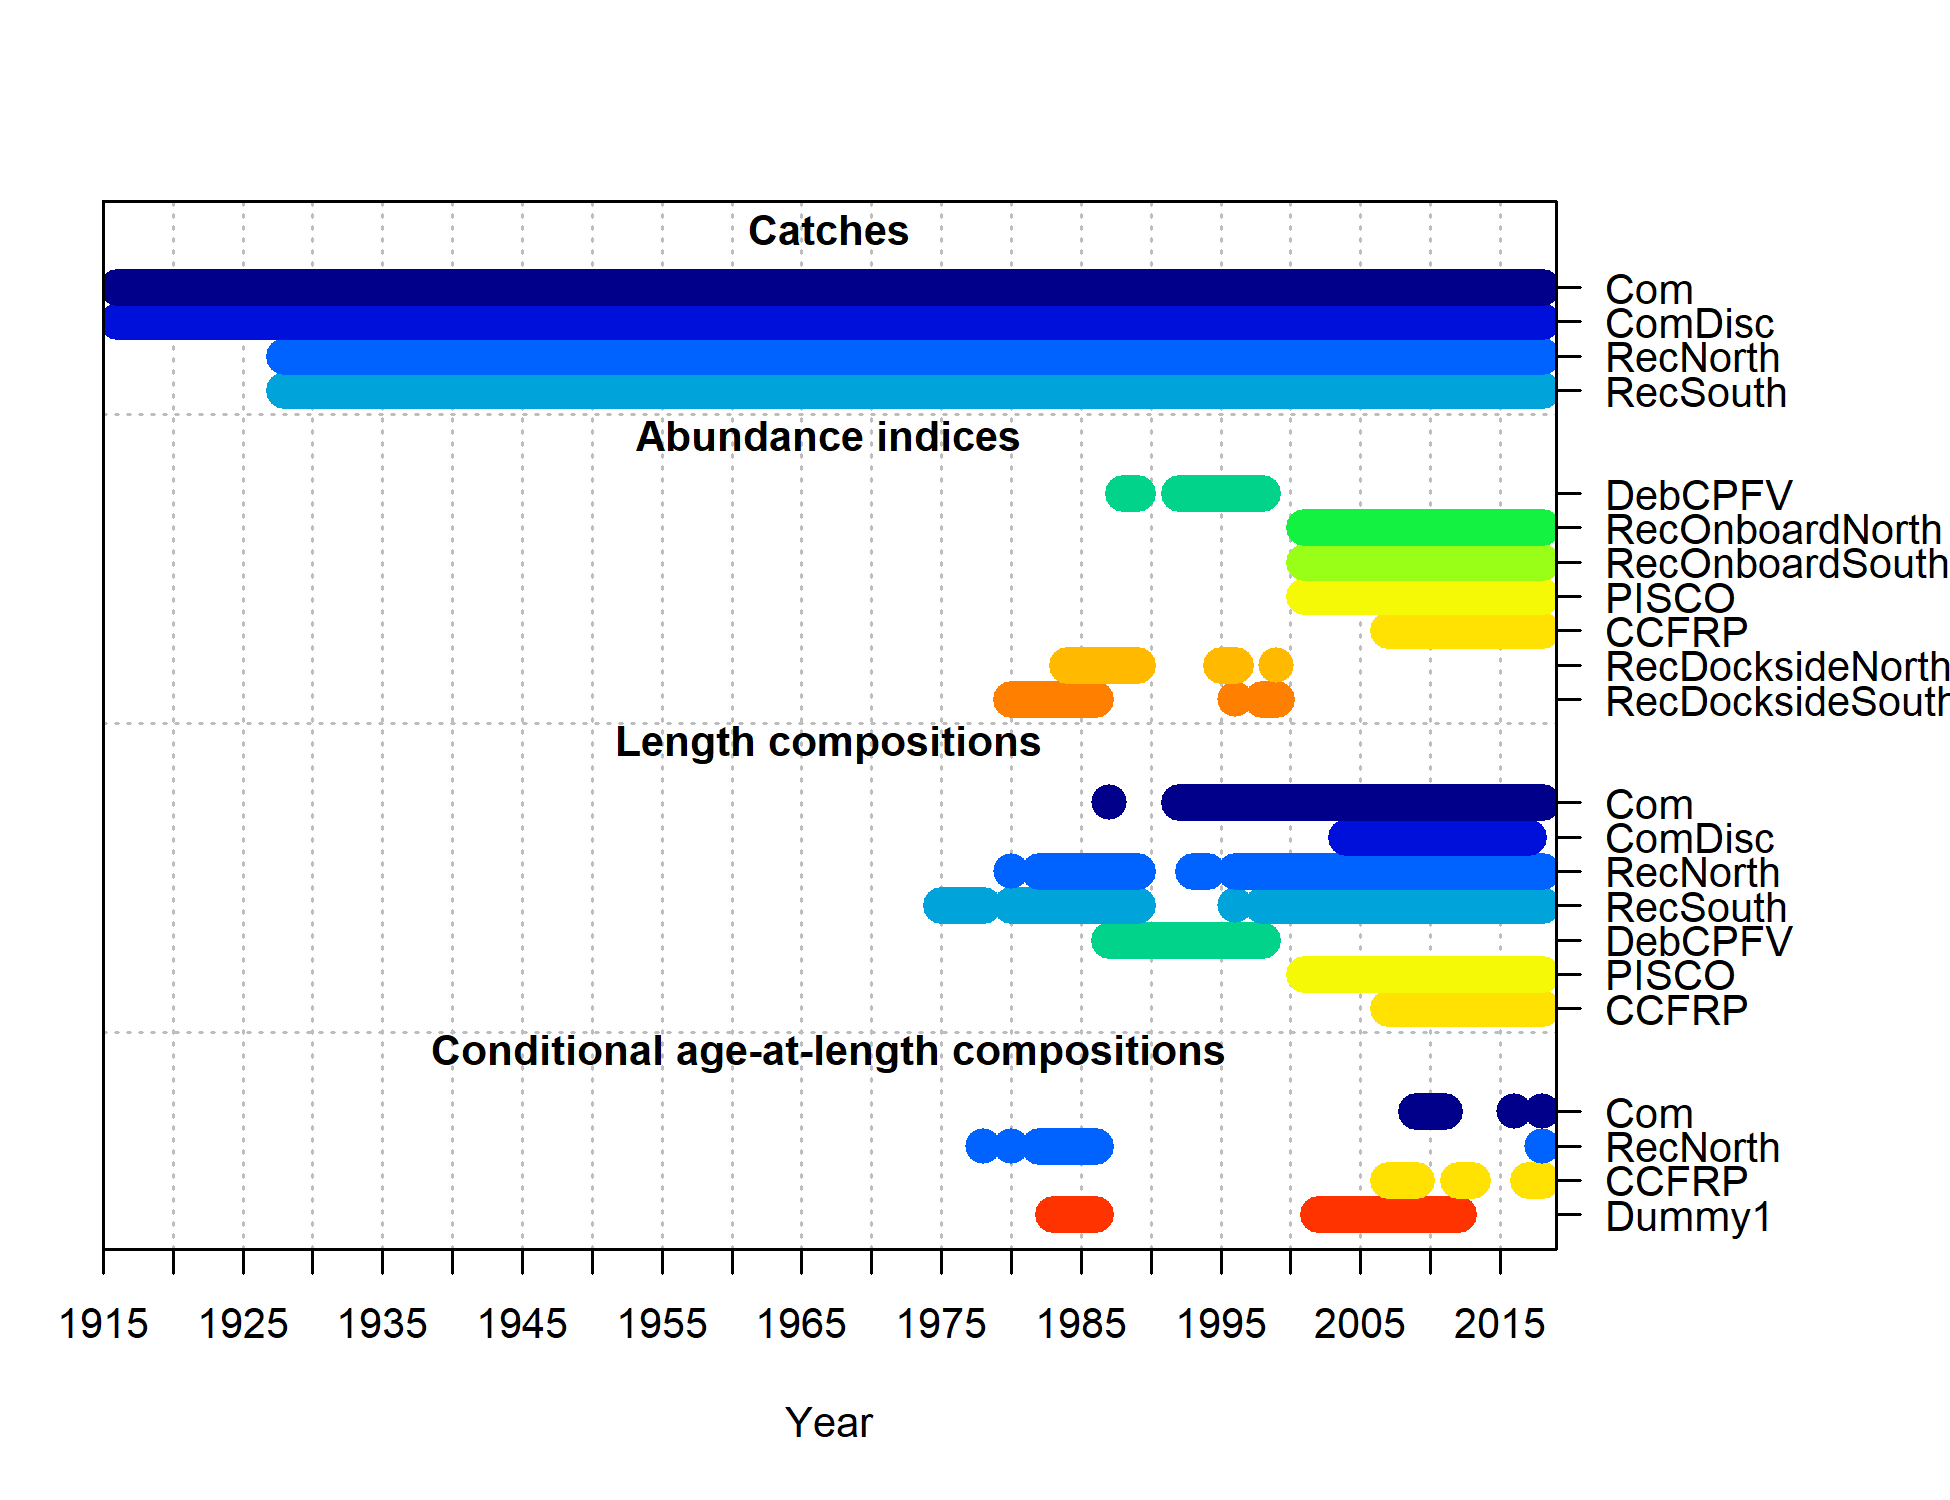
\includegraphics{r4ss/plots_mod1/data_plot.png}
\caption{Summary of data sources used in the model.
\label{fig:data_plot}}
\end{figure}

\begin{figure}
\centering
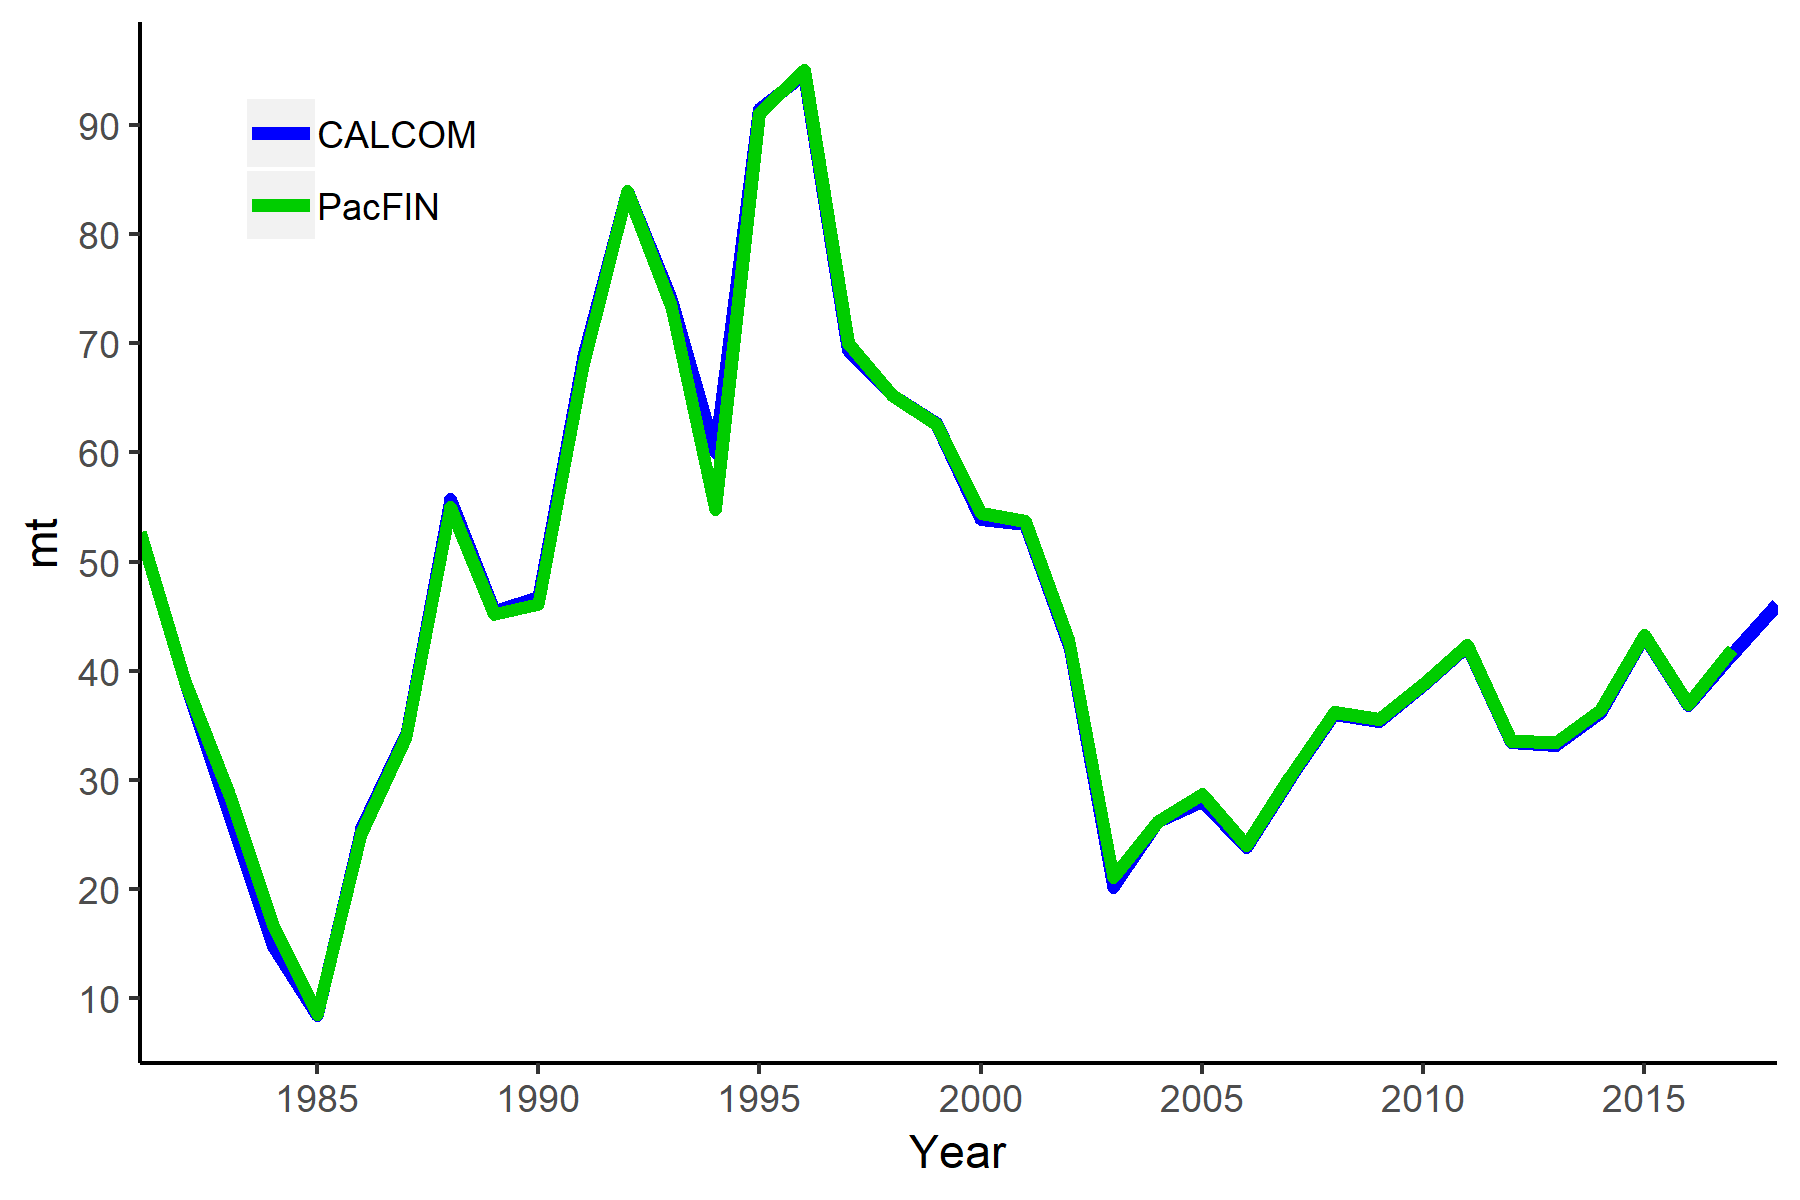
\includegraphics{Figures/Calcom_vs_Pacfin.png}
\caption{Commercial landings estimates from CALCOM add PacFIN.
\label{fig:Calcom_vs_Pacfin}}
\end{figure}

\begin{figure}
\centering
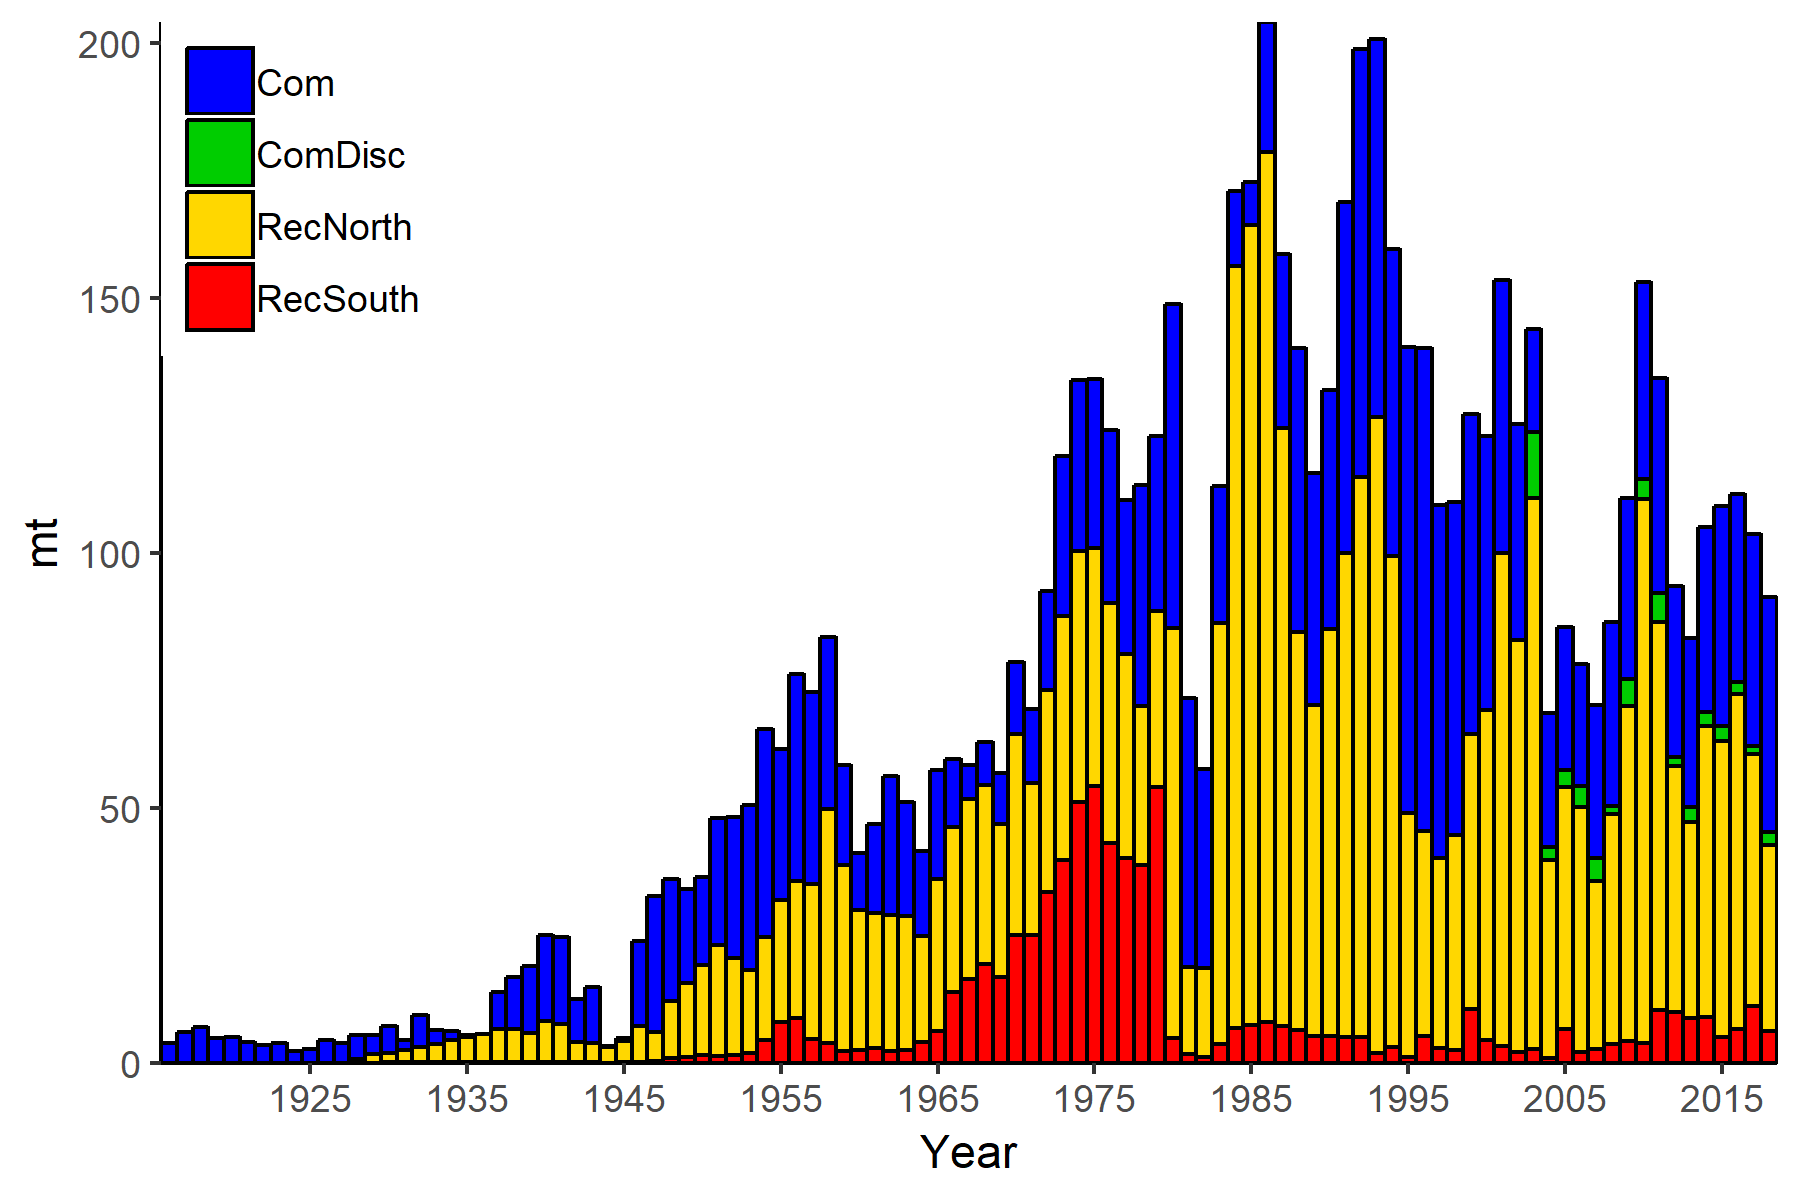
\includegraphics{Figures/Catches_original.png}
\caption{Commercial and recreational landings estimates prior to any
data modification or interpolation to the recreational catches or
hindcasting of commercial discards. \label{fig:Catches_original}}
\end{figure}

\begin{figure}
\centering
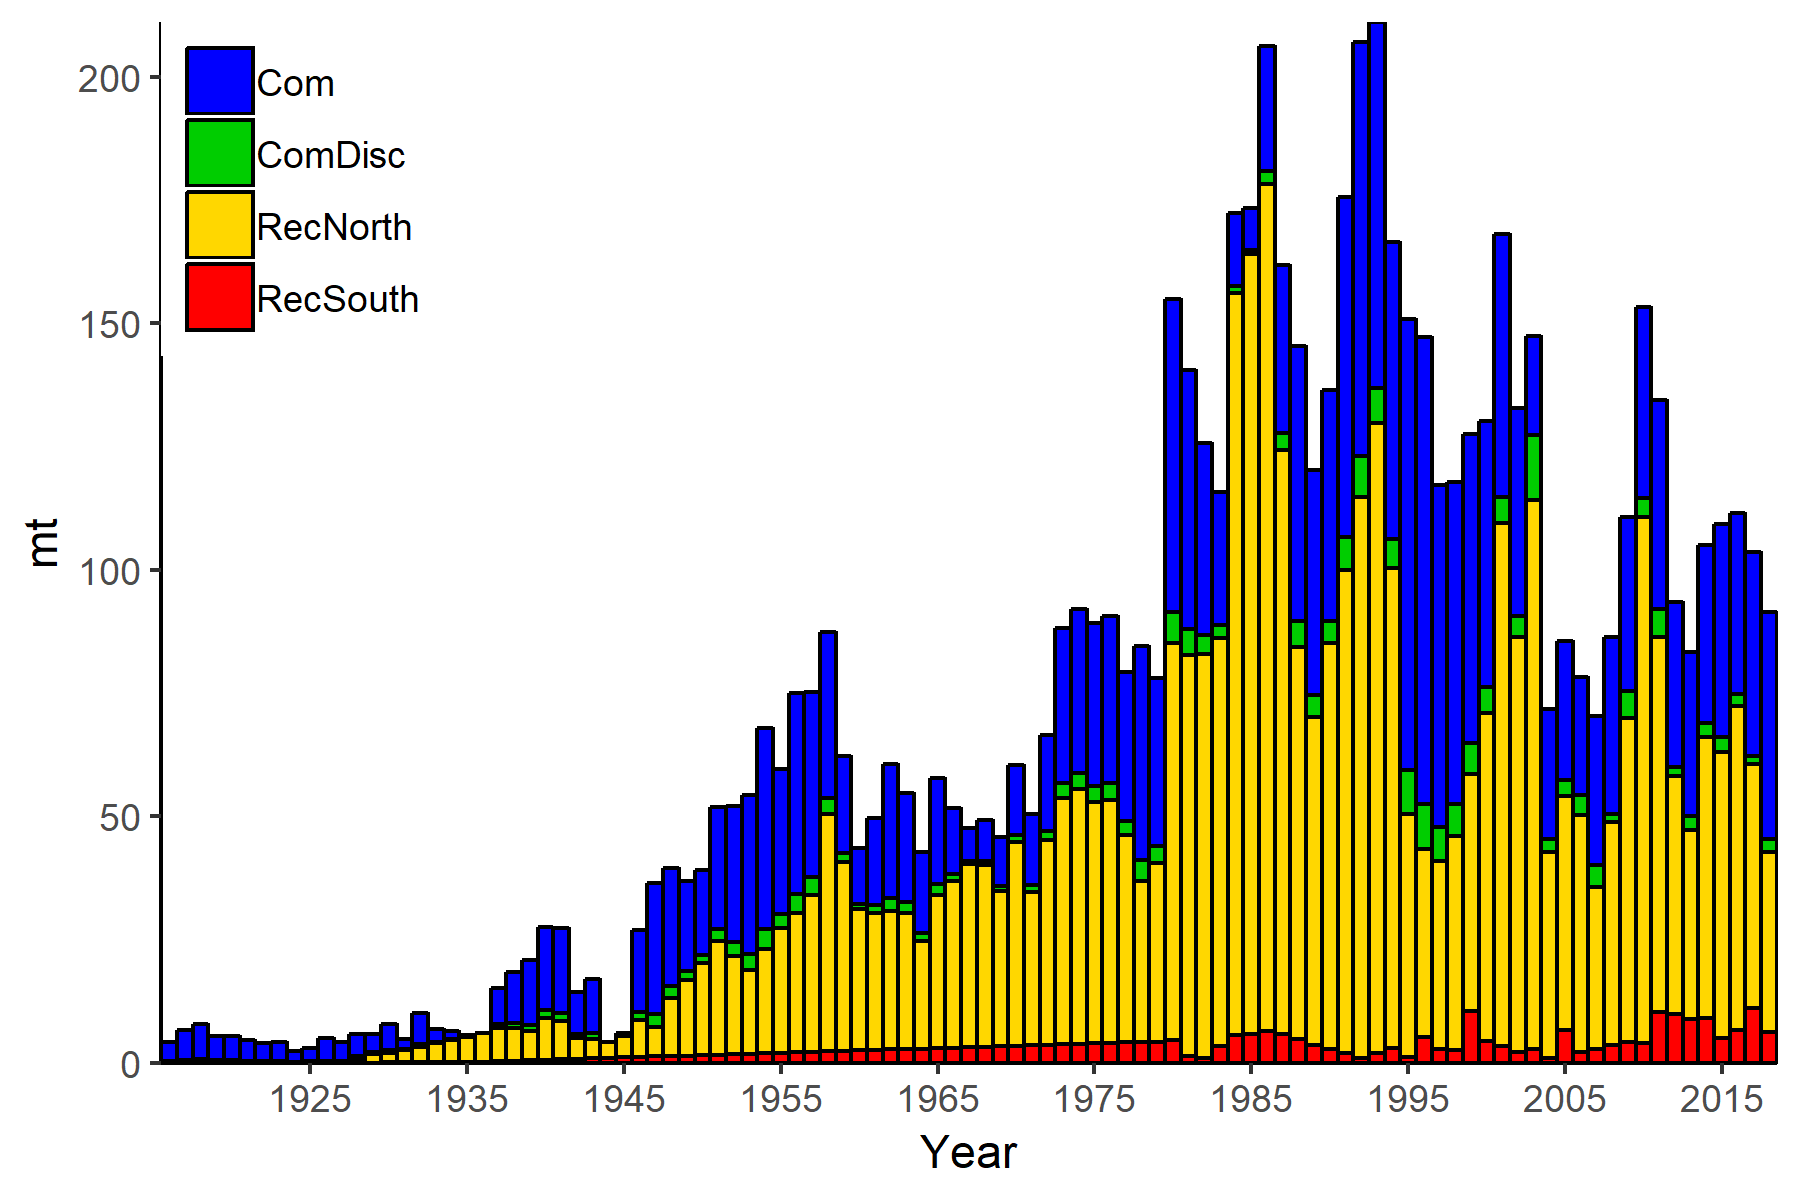
\includegraphics{Figures/Catches_alternate.png}
\caption{Commercial and recreational landings estimates after data
modification and interpolations were made to the recreational catches
and commercial discards. \label{fig:Catches_alternate}}
\end{figure}

\FloatBarrier

\FloatBarrier

\FloatBarrier
<!-- ********************************************************************** -->

\FloatBarrier

\FloatBarrier

\FloatBarrier

\FloatBarrier

\newpage

\color{black}

\section*{References}\label{references}
\addcontentsline{toc}{section}{References}

\renewcommand{\thepage}{}

\hypertarget{refs}{}
\hypertarget{ref-vonB1938}{}
Bertalanffy, L. von. 1938. A quantitative theory of organic growth.
Human Biology \textbf{10}: 181--213.

\hypertarget{ref-Hamel2015}{}
Hamel, O. 2015. A method for calculating a meta-analytical prior for the
natural mortality rate using multiple life history correlates. ICES
Journal of Marine Science \textbf{72}: 62--69.

\hypertarget{ref-PSMFC2018}{}
Pacific Fishery Managment Council. 2018. Status of the Pacific Coast
Groundfish Fishery: Stock Assessment and Fishery Evaluation.

\hypertarget{ref-Pearson2008}{}
Pearson, D.E., Erwin, B., and Key, M. 2008. Reliability of California's
groundfish landings estimates from 1969-2006. NOAA Technical Memorandum
NMFS \textbf{NOAA-TM-NM}.

\hypertarget{ref-Ralston2010}{}
Ralston, S., Pearson, D., Field, J., and Key, M. 2010. Documentation of
California catch reconstruction project. NOAA-TM-NMFS-SWFSC-461.

\hypertarget{ref-Somers2018}{}
Somers, K.A., J. Jannot, V. Tuttle, K. Richerson, N.R., and McVeigh, J.
2018. Estimated discard and catch of groundfish species in the 2017 US
west coast fisheries.. NOAA Fisheries, NWFSC Observer Program, 2725
Montlake Blvd E., Seattle, WA 98112.

\end{document}
